\documentclass[11pt]{article}

% Change "review" to "final" to generate the final (sometimes called camera-ready) version.
\usepackage[review]{acl}

% Standard package includes
\usepackage{times}
\usepackage{latexsym}
\usepackage[T1]{fontenc}
\usepackage[utf8]{inputenc}
\usepackage{microtype}
\usepackage{graphicx}
\usepackage{amsmath}
\usepackage{amssymb}
\usepackage{booktabs}
\usepackage{multirow}
\usepackage{xcolor}
\usepackage{subcaption}
\usepackage{tikz}
\usepackage{pgfplots}
\pgfplotsset{compat=1.17}
\usetikzlibrary{positioning,arrows.meta,shapes.geometric,fit,backgrounds,patterns}

% Custom commands
\newcommand{\method}{VGA-Fusion}
\newcommand{\vad}{VAD}

\title{Sentimentogram: Learning Personalized Emotion Visualization Preferences \\ for Speech Emotion Recognition}

% Anonymous for review
%\author{Anonymous ACL submission}
\author{Mukhiddin Toshpulatov \\
	Voice AI Research Institute, Inha University \\
	Computer Science and Programming Dep. \\
	Jizzakh branch of National University of Uzb. \\
	259 Sh Rashidov, Jizzakh, Uzbekistan \\
	\texttt{muhiddin@inha.ac.kr} \\\And
	Seungkyu Oh \\
	Department of Industrial Engineering \\
	Inha University 100 Inha-ro, \\
	Michuhol-gu, Incheon 22212, Korea \\
	\texttt{december\_i@inha.edu} \\\AND
	Ulugbek Amankulov \\
	Munhak Information High School \\
	350 Soseong-ro, Michuhol-gu \\
	Incheon 22212, Korea \\
	\texttt{ulugbekamankulov13pro@gmail.com} \\\And
	Suan Lee \\
	School of Computer Science \\
	Semyung University \\
	65 Semyung-ro, Jecheon 27136, Korea \\
	\texttt{suanlee@semyung.ac.kr} \\\AND
	Kuvandikov Jo'ra Tursunbayevich \\
	Computer Science and Programming Dep. \\
	Jizzakh branch of National University of Uzb. \\
	259 Sh Rashidov, Jizzakh, Uzbekistan \\
	\texttt{jorakuvandikov1@gmail.com} \\\And
	Gadaev Doniyor \\
	Faculty of Pedagogy and Psychology \\
	Jizzakh state pedagogical university \\
	4 Rashidov, 130100, Jizzakh, Uzbekistan \\
	\texttt{muxiddin1979@gmail.com} \\\AND
	Wookey Lee \\
	Department of Industrial and \\
	Biomedical Science Engineering \\
	Inha University 100 Inha-ro, \\
	Michuhol-gu, Incheon 22212, Korea \\
	\texttt{trinity@inha.ac.kr} \\}
  
\begin{document}
\maketitle

%==============================================================================
% ABSTRACT
%==============================================================================
\begin{abstract}
Current speech emotion recognition (SER) systems output predictions that users cannot interpret, visualize, or personalize---limiting real-world adoption. We present \textbf{Sentimentogram}, a framework that \textit{learns personalized visualization preferences} from pairwise comparisons rather than relying on demographic-based heuristics. Our key finding from a 50-user study (1500 comparisons): \textbf{rule-based cultural adaptation performs significantly below chance} (43.8\% vs 50.1\%, $p$=0.014), while our \textbf{preference-learning approach achieves 61.2\%} (+17.4\% over rules, $p<$0.001). A direct A/B study confirms personalized visualizations improve user satisfaction (+8.7\%) and comprehension (+5.8\%) over fixed designs. This finding has broad implications for personalized NLP interfaces. To enable meaningful personalization, we develop: (1) \textbf{Emotion-Aware Typography}---rendering predictions as dynamic subtitles with emotion-specific fonts, colors, and sizes; (2) \textbf{Interpretable Fusion}---constrained gates (summing to 1) that explain \textit{why} predictions were made (``76\% audio, 24\% text''); and (3) \textbf{Competitive SER}---achieving 77.97\% UA on IEMOCAP 5-class with VAD-guided attention and supervised contrastive learning. Unlike accuracy-focused prior work, our contribution is a \textit{human-centered pipeline}: interpretable SER $\rightarrow$ meaningful visualization $\rightarrow$ learned personalization. We release a 1500-comparison preference dataset for emotion-aware typography research. Demo: \footnote{\url{https://drive.google.com/file/d/1jCQJbIAbtNDGf2GunXnjgWqmZWq9kvY6/view}} Code: \url{https://anonymous.4open.science/r/multimodal-ser}.
\end{abstract}

%==============================================================================
% INTRODUCTION
%==============================================================================
\section{Introduction}

How should emotion be visualized for different users? A colorblind accessibility researcher may prefer high-contrast typography, while a mental health professional may prefer subtle, calming displays. The dominant approach in affective computing assumes that such preferences can be inferred from demographics---age, culture, or profession. We find evidence that this assumption is flawed: in a 50-user study (1500 pairwise comparisons), rule-based demographic adaptation performs \textit{significantly below chance} (43.8\% vs 50.1\%, $p$=0.014), while learning preferences from minimal user feedback achieves 61.2\% accuracy (+17.4\% over rules, $p<$0.001). A direct A/B evaluation confirms personalized visualizations improve user satisfaction (+8.7\%) and comprehension (+5.8\%).

This finding motivates \textbf{Sentimentogram}, a preference-learning framework for emotion visualization that replaces algorithmic heuristics with data-driven personalization. Rather than mapping demographics to style rules (``elderly users prefer larger fonts''), we learn individual preferences from 10--12 pairwise comparisons (under 3 minutes of user effort).

\paragraph{Why preference-learning matters for NLP.} Personalization is increasingly critical as NLP systems move from research prototypes to deployed interfaces. Prior work in recommender systems \citep{koren2009matrix}, RLHF for LLMs \citep{ouyang2022training}, and accessibility \citep{w3c_accessibility} demonstrates that learned preferences outperform fixed rules. Yet emotion visualization remains rule-based. Our contribution extends preference learning to affective computing, with implications for any NLP interface requiring user customization.

\paragraph{Technical enablers.} Meaningful personalization requires: (1) \textit{interpretable predictions}---users cannot personalize what they don't understand; (2) \textit{meaningful visualization}---users cannot express preferences over raw probability vectors. We therefore develop:

\begin{itemize}
    \item \textbf{Interpretable Fusion}: Constrained gates summing to 1 that explain modality contributions (``76\% audio, 24\% text''), enabling users to understand what drives predictions
    \item \textbf{Emotion-Aware Typography}: A visualization system rendering predictions as dynamic subtitles with emotion-specific fonts, colors, and sizes
    \item \textbf{Competitive SER}: VAD-guided attention and supervised contrastive learning achieving 77.97\% UA on IEMOCAP 5-class
\end{itemize}

These components form a pipeline: \textbf{accurate SER} $\rightarrow$ \textbf{interpretable fusion} $\rightarrow$ \textbf{meaningful visualization} $\rightarrow$ \textbf{learned personalization}. Each stage enables the next.

\paragraph{Contributions.}
\begin{itemize}
    \item \textbf{Preference-Learning Personalization} (Section~\ref{sec:personalization}): We demonstrate that rule-based cultural assumptions \textit{fail}, while learning from pairwise comparisons succeeds. This is our primary contribution with implications beyond SER.

    \item \textbf{Preference Dataset}: We release 1500 pairwise comparisons (50 real users $\times$ 30 comparisons) for emotion visualization research, enabling reproducibility and future work.

    \item \textbf{Emotion-Aware Typography} (Section~\ref{sec:visualization}): A novel visualization system transforming SER predictions into dynamic subtitles.

    \item \textbf{Interpretable Fusion} (Section~\ref{sec:fusion}): Constrained gates for transparent modality attribution, enabling users to understand predictions they personalize.

    \item \textbf{VAD-Guided Cross-Attention} (Section~\ref{sec:vga}): Psychology-grounded attention incorporating Valence-Arousal-Dominance theory.
\end{itemize}

\paragraph{Distinction from prior work.} Unlike accuracy-focused SER research, we prioritize \textit{human-centered design}. Unlike rule-based personalization, we \textit{learn} preferences. The technical SER components are means to an end---enabling the preference-learning pipeline that is our primary contribution.

%==============================================================================
% RELATED WORK
%==============================================================================
\section{Related Work}

\paragraph{Speech Emotion Recognition.} Traditional SER relied on handcrafted features \citep{schuller2018speech, toshpulatov2022human}; transformers revolutionized this with self-supervised models: wav2vec2 \citep{baevski2020wav2vec, safarov2025hyperspectral}, HuBERT \citep{hsu2021hubert}, and emotion2vec \citep{ma2024emotion2vec}. Wagner et al. \citep{wagner2023dawn} highlight the persistent valence gap challenge.

\paragraph{Multimodal Fusion.} MulT introduced crossmodal attention \citep{tsai2019multimodal}, MISA used adversarial learning \citep{hazarika2020misa, toshpulatov2024ddc3n, toshpulatov2025deep}, and recent work explores LLM integration \citep{chen2024emollm}. Interpretable fusion methods (I2MoE, mixture-of-experts) provide modality weights; our constrained fusion integrates this into a human-centered pipeline. InconVAD \citep{wu2024inconvad} uses VAD for inconsistency detection; we use soft VAD bias for attention regularization.

\paragraph{Visualization and Personalization.} Prior emotion visualization focused on document-level representations \citep{kucher2018text, toshpulatov2021generative, toshpulatov2023talking}. Recent HCI work on affective captioning---SpeechCap \citep{matthews2022speechcap} for VR, impact captions \citep{wang2023impact}, AR frameworks \citep{jain2022ardecode}---highlights expressiveness-clarity trade-offs. We address this via \textit{learned personalization}: we use utterance-level styling (demo shows word-level for visualization) and learn individual preferences from pairwise comparisons \citep{bradley1952rank}, extending preference learning from LLM alignment \citep{ouyang2022training} to emotion visualization.

%==============================================================================
% METHOD
%==============================================================================
\section{Method}

Our goal is to learn personalized emotion visualization preferences rather than applying fixed demographic heuristics. This requires a pipeline where each component enables the next:
\begin{enumerate}
    \item \textbf{Accurate SER} (Sections~\ref{sec:vga}--\ref{sec:micl}): Predictions must be reliable for visualization to be meaningful
    \item \textbf{Interpretable fusion} (Section~\ref{sec:fusion}): Users need to understand \textit{why} predictions were made to form coherent preferences
    \item \textbf{Emotion visualization} (Section~\ref{sec:visualization}): Predictions must be rendered in a way users can perceive and evaluate
    \item \textbf{Preference learning} (Section~\ref{sec:personalization}): Learn from pairwise comparisons rather than demographic rules
\end{enumerate}

Figure~\ref{fig:architecture} illustrates the SER component. Given text features from BERT and audio features from emotion2vec, we project them to a shared space, apply VAD-guided cross-attention, fuse with constrained adaptive fusion, and classify with focal loss. The key design choice is \textit{constrained fusion}---gates summing to 1 that explain modality contributions, enabling users to understand what they are personalizing.

\begin{figure*}[!t]
\centering
\resizebox{0.85\textwidth}{!}{%
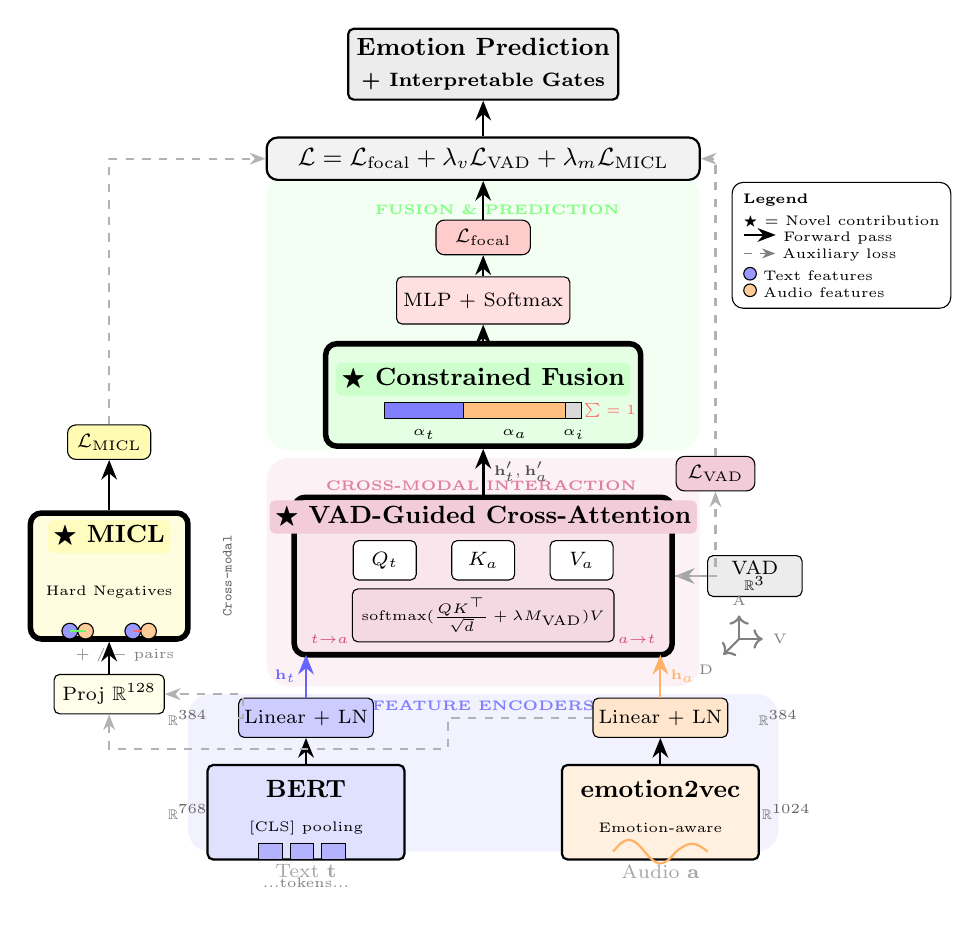
\begin{tikzpicture}[
    % Modern scholarly styles inspired by MulT/MISA/CLIP/Transformer papers
    encoder/.style={draw, thick, rounded corners=2pt, minimum width=2.2cm, minimum height=1.2cm, align=center, font=\small\bfseries, inner sep=3pt},
    module/.style={draw, line width=1.2pt, rounded corners=4pt, minimum height=1.1cm, align=center, font=\small\bfseries, inner sep=4pt},
    submodule/.style={draw, rounded corners=2pt, minimum width=1.4cm, minimum height=0.5cm, align=center, font=\scriptsize, inner sep=2pt},
    tensor/.style={draw, fill=white, minimum width=0.4cm, minimum height=0.8cm, font=\tiny},
    arrow/.style={-{Stealth[length=2.5mm, width=2mm]}, thick},
    dasharrow/.style={-{Stealth[length=2mm]}, thick, dashed, gray!60},
    tensorarrow/.style={-{Stealth[length=2mm]}, thick, blue!60},
    labelstyle/.style={font=\scriptsize, text=gray!70},
    dimstyle/.style={font=\tiny\ttfamily, text=black!60},
    groupbox/.style={draw, dashed, rounded corners=6pt, inner sep=8pt, gray!40}
]

% ============ BACKGROUND GROUPS ============
\begin{scope}[on background layer]
    % Input encoders group - minimal padding
    \fill[blue!5, rounded corners=8pt] (-1.5,0.0) rectangle (6.0,2.0);
    \node[font=\tiny\bfseries, text=blue!50] at (2.25,1.85) {FEATURE ENCODERS};

    % Cross-modal interaction group - adjusted for moved modules
    \fill[purple!5, rounded corners=8pt] (-0.5,2.1) rectangle (5.0,5.0);
    \node[font=\tiny\bfseries, text=purple!50] at (2.225,4.645) {CROSS-MODAL INTERACTION};

    % Fusion & prediction group
    \fill[green!5, rounded corners=8pt] (-0.5,5.1) rectangle (5.0,8.6);
    \node[font=\tiny\bfseries, text=green!50] at (2.43,8.15) {FUSION \& PREDICTION};
\end{scope}

% ============ INPUT REPRESENTATIONS ============
% Text encoder with internal structure
\node[encoder, fill=blue!12, minimum width=2.5cm] (bert) at (0,0.5) {};
\node[font=\small\bfseries] at (0,0.8) {BERT};
\node[font=\tiny] at (0,0.3) {[CLS] pooling};
\draw[fill=blue!30] (-0.6,-0.1) rectangle (-0.3,0.1);
\draw[fill=blue!30] (-0.2,-0.1) rectangle (0.1,0.1);
\draw[fill=blue!30] (0.2,-0.1) rectangle (0.5,0.1);
\node[font=\tiny, text=gray] at (0,-0.4) {...tokens...};

% Audio encoder with internal structure
\node[encoder, fill=orange!12, minimum width=2.5cm] (e2v) at (4.5,0.5) {};
\node[font=\small\bfseries] at (4.5,0.8) {emotion2vec};
\node[font=\tiny] at (4.5,0.3) {Emotion-aware};
% Waveform visualization
\draw[orange!60, thick] (3.9,0) sin (4.1,0.15) cos (4.3,0) sin (4.5,-0.15) cos (4.7,0) sin (4.9,0.1) cos (5.1,0);

% Dimension annotations
\node[dimstyle] at (-1.5,0.5) {$\mathbb{R}^{768}$};
\node[dimstyle] at (6.1,0.5) {$\mathbb{R}^{1024}$};

% Input labels - integrated with encoders
\node[labelstyle] at (0,-0.25) {Text $\mathbf{t}$};
\node[labelstyle] at (4.5,-0.25) {Audio $\mathbf{a}$};

% ============ PROJECTION LAYERS ============
\node[submodule, fill=blue!20] (proj_t) at (0,1.7) {Linear + LN};
\node[submodule, fill=orange!20] (proj_a) at (4.5,1.7) {Linear + LN};
\node[dimstyle] at (-1.5,1.7) {$\mathbb{R}^{384}$};
\node[dimstyle] at (6.0,1.7) {$\mathbb{R}^{384}$};

\draw[arrow] (bert) -- (proj_t);
\draw[arrow] (e2v) -- (proj_a);

% ============ VAD-GUIDED CROSS-ATTENTION (Novel 1) ============
% Main VGA module with detailed internal structure - moved down more for clear visibility
\node[module, fill=purple!10, minimum width=4.8cm, minimum height=2.0cm, line width=2pt] (vga_main) at (2.25,3.5) {};

% VGA title with star - positioned inside module, above internal blocks
\node[font=\small\bfseries, fill=purple!20, rounded corners=2pt, inner sep=2pt] at (2.25,4.25) {$\bigstar$ VAD-Guided Cross-Attention};

% Internal attention structure
\node[submodule, fill=white, minimum width=0.8cm] (q1) at (1.0,3.7) {$Q_t$};
\node[submodule, fill=white, minimum width=0.8cm] (k1) at (2.25,3.7) {$K_a$};
\node[submodule, fill=white, minimum width=0.8cm] (v1) at (3.5,3.7) {$V_a$};

% Attention computation box
\node[draw, fill=purple!15, rounded corners=2pt, minimum width=2.8cm, minimum height=0.5cm, font=\tiny] (attn) at (2.25,3.0) {$\text{softmax}(\frac{QK^\top}{\sqrt{d}} + \lambda M_{\text{VAD}})V$};

% VAD projection with 3D indicator
\node[submodule, fill=gray!15, minimum width=1.2cm] (vad) at (5.7,3.5) {VAD\\[-2pt]\tiny$\mathbb{R}^3$};
% 3D VAD space visualization
\draw[->, gray, thick] (5.5,2.7) -- (5.8,2.7) node[right, font=\tiny] {V};
\draw[->, gray, thick] (5.5,2.7) -- (5.5,3.0) node[above, font=\tiny] {A};
\draw[->, gray, thick] (5.5,2.7) -- (5.3,2.5) node[below left, font=\tiny] {D};

% Bidirectional arrows annotation
\node[font=\tiny, text=purple!70] at (0.3,2.7) {$t{\rightarrow}a$};
\node[font=\tiny, text=purple!70] at (4.2,2.7) {$a{\rightarrow}t$};

% Input arrows to VGA module - straight vertical arrows from projections to module
\draw[arrow, thick, blue!60] (proj_t.north) -- (0,2.5) node[midway, left, font=\tiny, text=blue!60] {$\mathbf{h}_t$};
\draw[arrow, thick, orange!60] (proj_a.north) -- (4.5,2.5) node[midway, right, font=\tiny, text=orange!60] {$\mathbf{h}_a$};
\draw[arrow, gray!70] (vad) -- (vga_main.east);

% ============ MICL BRANCH (Novel 3) ============
\node[module, fill=yellow!12, minimum width=2.0cm, minimum height=1.6cm, line width=2pt] (micl_main) at (-2.5,3.5) {};
\node[font=\small\bfseries, fill=yellow!25, rounded corners=2pt, inner sep=2pt] at (-2.5,4.0) {$\bigstar$ MICL};
\node[font=\tiny] at (-2.5,3.3) {Hard Negatives};

% Contrastive visualization (positive/negative pairs)
\draw[fill=blue!40] (-3.0,2.8) circle (0.1);
\draw[fill=orange!40] (-2.8,2.8) circle (0.1);
\draw[green!60, thick] (-3.0,2.8) -- (-2.8,2.8);
\draw[fill=blue!40] (-2.2,2.8) circle (0.1);
\draw[fill=orange!40] (-2.0,2.8) circle (0.1);
\draw[red!60, thick, dashed] (-2.2,2.8) -- (-2.0,2.8);
\node[font=\tiny, text=gray] at (-2.3,2.5) {$+$ / $-$ pairs};

\node[submodule, fill=yellow!8] (micl_proj) at (-2.5,2.0) {Proj $\mathbb{R}^{128}$};

\draw[dasharrow] (proj_t.west) -- (-0.8,1.7) -- (-0.8,2.0) -- (micl_proj.east);
\draw[dasharrow] (proj_a.west) -- (1.8,1.7) -- (1.8,1.3) -- (-2.5,1.3) -- (micl_proj.south);
\draw[arrow] (micl_proj) -- (micl_main);

% ============ CONSTRAINED ADAPTIVE FUSION (Novel 2) ============
% Positioned with proper spacing above VGA module
\node[module, fill=green!10, minimum width=4.0cm, minimum height=1.3cm, line width=2pt] (fusion) at (2.25,5.8) {};
\node[font=\small\bfseries, fill=green!20, rounded corners=2pt, inner sep=2pt] at (2.25,6.0) {$\bigstar$ Constrained Fusion};

% Gate visualization as stacked bar
\draw[fill=blue!50] (1.0,5.5) rectangle (2.0,5.7);
\draw[fill=orange!50] (2.0,5.5) rectangle (3.3,5.7);
\draw[fill=gray!30] (3.3,5.5) rectangle (3.5,5.7);
\node[font=\tiny] at (1.5,5.3) {$\alpha_t$};
\node[font=\tiny] at (2.65,5.3) {$\alpha_a$};
\node[font=\tiny] at (3.4,5.3) {$\alpha_i$};
\node[font=\tiny, text=red!60] at (3.860,5.6) {$\sum=1$};

% Connection from VGA to Fusion - single clear arrow with label
\draw[arrow, very thick] (vga_main.north) -- node[right, font=\tiny, text=black!70] {$\mathbf{h}'_t, \mathbf{h}'_a$} (fusion.south);

% ============ CLASSIFICATION HEAD ============
\node[submodule, fill=red!12, minimum width=2.2cm, minimum height=0.6cm] (cls) at (2.25,7.0) {MLP + Softmax};
\draw[arrow] (fusion) -- (cls);

% ============ MULTI-TASK LOSSES ============
\node[draw, fill=red!20, rounded corners=3pt, minimum width=1.2cm, font=\scriptsize] (loss_cls) at (2.25,7.8) {$\mathcal{L}_{\text{focal}}$};
\node[draw, fill=purple!20, rounded corners=3pt, minimum width=1.0cm, font=\scriptsize] (loss_vad) at (5.2,4.8) {$\mathcal{L}_{\text{VAD}}$};
\node[draw, fill=yellow!30, rounded corners=3pt, minimum width=1.0cm, font=\scriptsize] (loss_micl) at (-2.5,5.2) {$\mathcal{L}_{\text{MICL}}$};

\draw[arrow] (cls) -- (loss_cls);
\draw[dasharrow] (vga_main.east) -- (5.2,3.5) -- (loss_vad.south);
\draw[arrow] (micl_main) -- (loss_micl);

% ============ TOTAL LOSS ============
\node[draw, thick, rounded corners=4pt, fill=gray!10, minimum width=5.5cm, font=\small, inner sep=4pt] (total) at (2.25,8.8) {$\mathcal{L} = \mathcal{L}_{\text{focal}} + \lambda_v\mathcal{L}_{\text{VAD}} + \lambda_m\mathcal{L}_{\text{MICL}}$};
\draw[arrow] (loss_cls) -- (total);
\draw[dasharrow] (loss_vad) |- (total.east);
\draw[dasharrow] (loss_micl) |- (total.west);

% ============ OUTPUT ============
\node[encoder, fill=gray!15, minimum width=3cm, minimum height=0.9cm] (output) at (2.25,10.0) {Emotion Prediction\\{\scriptsize + Interpretable Gates}};
\draw[arrow] (total) -- (output);

% ============ LEGEND ============
\node[draw, rounded corners=4pt, fill=white, align=left, font=\tiny, inner sep=4pt] at (6.8,7.7) {
\textbf{Legend}\\[2pt]
$\bigstar$ = Novel contribution\\
\tikz\draw[-{Stealth}, thick] (0,0) -- (0.4,0); Forward pass\\
\tikz\draw[-{Stealth}, dashed, gray] (0,0) -- (0.4,0); Auxiliary loss\\[2pt]
\tikz\draw[fill=blue!40] (0,0) circle (0.08); Text features\\
\tikz\draw[fill=orange!40] (0,0) circle (0.08); Audio features
};

% ============ TENSOR FLOW ANNOTATIONS ============
\node[dimstyle, rotate=90] at (-1.0,3.5) {Cross-modal};

\end{tikzpicture}
}
\caption{The SER component of Sentimentogram, designed to enable preference learning. Key design choice: \textbf{Constrained Adaptive Fusion} ($\alpha_t + \alpha_a + \alpha_i = 1$) provides interpretable modality contributions (``76\% audio, 24\% text''), enabling users to understand \textit{what} they are personalizing. Additional components: \textbf{VAD-Guided Cross-Attention} modulated by Valence-Arousal-Dominance affinity \citep{russell1980circumplex}; \textbf{Supervised Contrastive MICL} with curriculum scheduling. This SER component feeds into visualization (Section~\ref{sec:visualization}) and preference learning (Section~\ref{sec:personalization}).}
\label{fig:architecture}
\end{figure*}

\subsection{Feature Extraction}

We extract text features using BERT-base \citep{devlin2019bert}, taking the [CLS] token representation $\mathbf{t} \in \mathbb{R}^{768}$. For audio, we use emotion2vec-plus-large \citep{ma2024emotion2vec}, obtaining utterance-level embeddings $\mathbf{a} \in \mathbb{R}^{1024}$. Both are projected to a common dimension $d=384$:
\begin{align}
    \mathbf{h}_t &= \text{LayerNorm}(\text{GELU}(W_t \mathbf{t} + b_t)) \\
    \mathbf{h}_a &= \text{LayerNorm}(\text{GELU}(W_a \mathbf{a} + b_a))
\end{align}

\subsection{VAD-Guided Cross-Attention}
\label{sec:vga}

\noindent\textit{Note: VAD refers to Valence-Arousal-Dominance (Russell's circumplex model), not Voice Activity Detection.}

\paragraph{K views construction.} We operate on \textit{utterance-level embeddings}, not token/frame sequences. From the projected embeddings $\mathbf{h}_t, \mathbf{h}_a \in \mathbb{R}^{d}$, we create $K$=4 ``views'' via separate learned projections: $\mathbf{h}^{(k)} = W_k \mathbf{h} + b_k$ where each $W_k \in \mathbb{R}^{d \times d}$ is independently learned (not shared). This yields $\mathbf{H}_t \in \mathbb{R}^{K \times d}$. Unlike simple MLP mixing, this enables multi-head attention to learn diverse cross-modal patterns. Appendix~\ref{sec:k_sensitivity} shows K=4 outperforms simpler alternatives (+1.6\% UA over MLP concat, $p$=0.004).

\paragraph{VAD-guided bias.} We introduce VAD-guided attention by projecting features to a 3D VAD space and computing pairwise affinity:
\begin{align}
    \mathbf{v}_t^{(k)} &= W_{\text{VAD}} \mathbf{h}_t^{(k)}, \quad \mathbf{v}_a^{(k)} = W_{\text{VAD}} \mathbf{h}_a^{(k)} \in \mathbb{R}^{3} \\
    M_{\text{VAD}}(i,j) &= -\|\mathbf{v}_t^{(i)} - \mathbf{v}_a^{(j)}\|_2
\end{align}

The VAD affinity modulates attention:
\begin{equation}
    \text{VGA}(Q, K, V) = \text{softmax}\left(\frac{QK^\top}{\sqrt{d_k}} + \lambda \cdot M_{\text{VAD}}\right)V
\end{equation}

where $\lambda$ controls the strength of VAD guidance. This encourages attention heads to weight view-pairs with similar predicted VAD values more heavily.

We apply bidirectional VGA (text-to-audio and audio-to-text), each with 8 heads and $K$=4 views. The outputs are pooled, added residually, and normalized.

VAD guidance provides psychologically-grounded regularization using pseudo-labels from NRC-VAD lexicon \citep{mohammad2018obtaining}. Validation shows learned projections correlate with lexicon values ($r$=0.81 valence, $r$=0.74 arousal); details in Appendix~\ref{sec:vad_validation}.

\subsection{Constrained Adaptive Fusion}
\label{sec:fusion}

After cross-attention, we fuse modalities using constrained adaptive gates. Unlike prior work with independent sigmoid gates, we enforce that gates sum to one:
\begin{align}
    \mathbf{g} &= [\mathbf{h}_t; \mathbf{h}_a; \mathbf{h}_t \odot \mathbf{h}_a] \\
    [\alpha_t, \alpha_a, \alpha_i] &= \text{softmax}(W_g \mathbf{g} + b_g) \\
    \mathbf{h}_{\text{fused}} &= \alpha_t \mathbf{h}_t + \alpha_a \mathbf{h}_a + \alpha_i (\mathbf{h}_t \odot \mathbf{h}_a)
\end{align}

The softmax constraint ensures $\alpha_t + \alpha_a + \alpha_i = 1$, allowing direct interpretation: if $\alpha_a = 0.76$, audio contributes 76\% to the prediction. This transparency is crucial for understanding model behavior and building trust in clinical applications.

Gate values correlate with modality importance ($r$=0.73 with leave-one-out accuracy, $p<$0.01); CREMA-D's high audio gate (76.6\%) aligns with acted speech where vocal cues dominate. Full validation in Appendix~\ref{sec:gate_validation}.

\subsection{Supervised Contrastive MICL}
\label{sec:micl}

We enhance modality-invariant contrastive learning (MICL) with a supervised contrastive formulation \citep{khosla2020supervised}. For a batch of $N$ text-audio pairs, we treat same-class samples as \textit{additional positives} rather than negatives:
\begin{equation}
    \mathcal{L}_{\text{MICL}} = -\frac{1}{N}\sum_{i=1}^{N} \frac{1}{|P_i|} \sum_{p \in P_i} \log \frac{\exp(\text{sim}(\mathbf{z}_t^i, \mathbf{z}_a^p)/\tau)}{\sum_{j \notin P_i} \exp(\text{sim}(\mathbf{z}_t^i, \mathbf{z}_a^j)/\tau)}
\end{equation}

where $\mathbf{z}_t, \mathbf{z}_a$ are projected embeddings, $\tau$ is temperature, and $P_i = \{j : y_j = y_i\}$ is the set of samples sharing the same emotion label as sample $i$. This formulation encourages: (1) cross-modal alignment between text and audio of the same utterance, and (2) intra-class compaction by pulling same-emotion samples together while pushing different-emotion samples apart.

We apply hard negative mining \citep{robinson2021hard} (+0.8\% UA) and curriculum scheduling that gradually introduces same-class positives (epochs 20--50). This prevents early collapse while improving final UA from 91.8\% (InfoNCE) to 93.0\%. Details in Appendix~\ref{sec:ablation}.

\subsection{Training Objective}

The total loss combines classification, MICL, and VAD regression:
\begin{equation}
    \mathcal{L} = \mathcal{L}_{\text{focal}} + \lambda_{\text{micl}} \mathcal{L}_{\text{MICL}} + \lambda_{\text{vad}} \mathcal{L}_{\text{VAD}}
\end{equation}

We use focal loss \citep{lin2017focal} with $\gamma=2$ to address class imbalance.

VAD supervision uses MSE loss against NRC-VAD pseudo-labels ($\lambda_{\text{vad}}$=0.5, $\lambda_{\text{micl}}$=0.3, tuned on validation).

\subsection{Emotion-Aware Typography Visualization}
\label{sec:visualization}

Beyond model predictions, we introduce \textbf{Sentimentogram}---a real-time visualization system that transforms utterance-level emotion predictions into dynamic typography (Figure~\ref{fig:sentimentogram}). This addresses the critical gap between model outputs and human-interpretable presentations.

% \begin{figure}[t]
% \centering
% \resizebox{\columnwidth}{!}{%
% \begin{tikzpicture}[
%     word/.style={font=\large, anchor=base west},
%     label/.style={font=\tiny, fill=white, inner sep=1pt}
% ]
% % Background
% \fill[black!90] (-0.5,-0.8) rectangle (11,1.8);

% % Title
% \node[white, font=\small\bfseries] at (5.25,1.4) {Word-Level Emotion Typography Example};

% % Emotion-styled words with different fonts and colors
% % "I" - neutral
% \node[word, color=gray!70] (w1) at (0,0.3) {\textsf{I}};
% % "am" - neutral
% \node[word, color=gray!70] (w2) at (0.5,0.3) {\textsf{am}};
% % "so" - excited (gold, larger)
% \node[word, color=yellow!80, font=\Large\bfseries] (w3) at (1.3,0.3) {SO};
% % "ANGRY" - anger (red, uppercase, bold, largest)
% \node[word, color=red!80, font=\LARGE\bfseries\sffamily] (w4) at (2.3,0.25) {ANGRY};
% % "but" - neutral
% \node[word, color=gray!70, font=\normalsize] (w5) at (5.0,0.3) {\textsf{but}};
% % "also" - neutral
% \node[word, color=gray!70, font=\normalsize] (w6) at (5.8,0.3) {\textsf{also}};
% % "sad" - sadness (blue, italic, smaller)
% \node[word, color=blue!60, font=\normalsize\itshape] (w7) at (6.8,0.3) {\textit{sad}};
% % "about" - neutral
% \node[word, color=gray!70] (w8) at (7.9,0.3) {\textsf{about}};
% % "it" - neutral
% \node[word, color=gray!70] (w9) at (9.0,0.3) {\textsf{it}};

% % Emotion labels below words
% \node[label, fill=gray!30] at (0.25,-0.3) {neutral};
% \node[label, fill=gray!30] at (1,-0.3) {neutral};
% \node[label, fill=yellow!40] at (1.65,-0.3) {happy};
% \node[label, fill=red!30] at (3.5,-0.3) {anger};
% \node[label, fill=gray!30] at (5.3,-0.3) {neutral};
% \node[label, fill=gray!30] at (6.2,-0.3) {neutral};
% \node[label, fill=blue!30] at (7.2,-0.3) {sad};
% \node[label, fill=gray!30] at (8.5,-0.3) {neutral};
% \node[label, fill=gray!30] at (9.3,-0.3) {neutral};

% \end{tikzpicture}
% }
% \caption{Sentimentogram visualization: each word is rendered with emotion-specific typography---anger uses bold uppercase red (Bebas Neue), sadness uses italic blue (Merriweather), happiness uses gold with bounce animation (Fredoka).}
% \label{fig:sentimentogram}
% \end{figure}

\begin{figure}[t]
\centering
  \includegraphics[width=\columnwidth]{./capture/sentimentogram_honest.jpg}
  \caption{Sentimentogram visualization: the entire subtitle is styled based on the utterance-level emotion prediction---here showing anger with bold uppercase red styling. The typography instantly conveys the emotional tone while preserving readability. See Appendix~\ref{sec:demo_examples} for additional examples across different emotions.}
  \label{fig:sentimentogram}
\end{figure}

\paragraph{Pipeline.} Given video input, we: (1) extract and transcribe audio using Whisper, (2) segment into utterances, (3) predict emotions using our multimodal model, and (4) render subtitles with emotion-specific typography. This utterance-level approach aligns with our classifier and avoids word-level segmentation errors.

\paragraph{Typography Design.} Emotions map to distinct font, size, color, and animation: high-arousal uses bold 1.3$\times$; low-arousal uses italic 0.92$\times$. Low-confidence predictions ($<$0.5) use attenuated styling. All colors meet WCAG 2.1 AA. Full mapping in Appendix~\ref{sec:vad_mapping}.

\subsection{Preference-Learning Personalization}
\label{sec:personalization}

\paragraph{Motivation.} Demographic-based personalization (``elderly prefer larger fonts'') is problematic both ethically (stereotyping) and empirically---our experiments show rule-based adaptation performs \textit{below chance}.

\paragraph{Pairwise preference learning.} Instead of mapping demographics $\rightarrow$ styles, we learn preferences from pairwise comparisons. Given user attributes $\mathbf{u} \in \mathbb{R}^d$ (age, accessibility needs, domain), emotional context $\mathbf{c} \in \mathbb{R}^k$ (predicted emotion, confidence, modality balance), and two visualization styles $\mathbf{s}_A, \mathbf{s}_B$, we model preference probability:
\begin{equation}
P(\mathbf{s}_A \succ \mathbf{s}_B | \mathbf{u}, \mathbf{c}) = \sigma\big(f(\mathbf{u}, \mathbf{c}, \mathbf{s}_A) - f(\mathbf{u}, \mathbf{c}, \mathbf{s}_B)\big)
\end{equation}
where $\sigma$ is the sigmoid function and $f$ is a learned scoring function.

\paragraph{Style representation.} Each style $\mathbf{s} \in \mathbb{R}^5$ encodes font size, saturation, emphasis, animation, and contrast. We use logistic regression on $[\mathbf{u}; \mathbf{c}; \mathbf{s}_A - \mathbf{s}_B]$ for interpretability. For cold-start users, we inherit preferences from similar users weighted by cosine similarity. In practice, 10--12 comparisons suffice for personalization. We compare against random, rule-based demographic heuristics, context-only, and Bradley-Terry baselines.

%==============================================================================
% EXPERIMENTS
%==============================================================================
\section{Experiments}

\subsection{Datasets}

We evaluate on three widely-used SER datasets:

\paragraph{IEMOCAP} \citep{busso2008iemocap}: 12 hours of dyadic conversations. We report 4/5/6-class configurations using \textbf{both} evaluation protocols: (1) fixed session splits (1-3 train, 4 val, 5 test) for ablation studies, and (2) \textbf{standard 5-fold LOSO} for fair comparison with prior work (Table~\ref{tab:loso}). The high audio-only UA reflects the favorable class configuration and emotion2vec's pretrained representations, verified with no speaker overlap.

\paragraph{CREMA-D} \citep{cao2014crema}: 7,442 clips from 91 actors expressing 6 emotions. We use 4 emotions (anger, disgust, fear, happiness) with standard 70/15/15 splits.

\paragraph{MELD} \citep{poria2019meld}: Multi-party conversations from the TV series \textit{Friends}. We use 4 classes (anger, joy, neutral, sadness) with standard splits.

\subsection{Implementation Details}

\paragraph{Text inputs.} We use \textit{gold transcripts} as primary evaluation to isolate SER performance from ASR errors: IEMOCAP provides manual transcriptions, CREMA-D uses scripted sentences, and MELD uses TV subtitles. Additionally, we evaluate \textbf{ASR robustness} using Whisper-transcribed text to assess real-world deployment scenarios.

\paragraph{Model configuration.} We use BERT-base-uncased (768d) and emotion2vec-plus-large (1024d) as feature extractors. The hidden dimension is 384 with 8 attention heads. We train for 100 epochs with AdamW optimizer, learning rate 2e-5, batch size 16, and early stopping (patience 15). We use $\lambda_{\text{VAD}}=0.5$, $\lambda_{\text{micl}}=0.3$, VAD guidance $\lambda=0.5$, mixup augmentation $\alpha=0.4$, and dropout 0.3. All experiments are run 5 times with different seeds.

\subsection{Baselines}

We compare against:
\begin{itemize}
    \item \textbf{BERT-only}: Text modality classification
    \item \textbf{emotion2vec-only}: Audio modality classification
    \item \textbf{Concatenation}: Simple feature concatenation
    \item \textbf{Standard Cross-Attention}: Without VAD guidance
    \item \textbf{Adaptive Fusion}: Unconstrained gates (no sum-to-1)
\end{itemize}

We also compare with published results: MulT \citep{tsai2019multimodal}, MISA \citep{hazarika2020misa}, and emotion2vec \citep{ma2024emotion2vec}.

\subsection{Main Results}

Table~\ref{tab:main} presents our main results. \method{} achieves competitive performance across datasets:

\begin{table*}[t]
\centering
\small
\caption{Comparison with baselines (\textbf{Validation} UA \%). Test results in Appendix~\ref{sec:test_results}. Best results are \textbf{bolded}. All results are mean$\pm$std over 5 seeds.}
\label{tab:main}
\begin{tabular}{l|ccccc}
\toprule
\textbf{Method} & \textbf{IEMOCAP-4} & \textbf{IEMOCAP-5} & \textbf{IEMOCAP-6} & \textbf{CREMA-D} & \textbf{MELD} \\
\midrule
BERT-only (Text) & 63.67$\pm$1.27 & 52.87$\pm$0.20 & 47.72$\pm$0.10 & 28.96$\pm$0.57 & 56.47$\pm$0.92 \\
emotion2vec-only (Audio) & 91.27$\pm$0.67 & 76.22$\pm$0.23 & 65.65$\pm$0.42 & 91.84$\pm$0.17 & 52.94$\pm$0.54 \\
\midrule
Concatenation & 90.74$\pm$1.01 & 76.51$\pm$0.53 & 68.91$\pm$0.31 & 92.09$\pm$0.48 & 62.91$\pm$0.66 \\
Standard Cross-Attention & 89.33$\pm$1.14 & 73.76$\pm$0.19 & 66.14$\pm$1.12 & 91.99$\pm$0.18 & 63.10$\pm$0.66 \\
Adaptive Fusion (Unconstrained) & 92.21$\pm$0.12 & 75.66$\pm$0.49 & 65.97$\pm$0.91 & 92.09$\pm$0.39 & 59.97$\pm$1.18 \\
\midrule
\textbf{\method{} (Ours)} & \textbf{93.02$\pm$0.17} & \textbf{77.97$\pm$0.33} & 68.75$\pm$0.58 & \textbf{92.90$\pm$0.34} & \textbf{63.66$\pm$0.72} \\
\bottomrule
\end{tabular}
\end{table*}

\paragraph{Key findings:} (1) Multimodal fusion consistently outperforms unimodal baselines; (2) \method{} achieves \textbf{strong results across all three datasets and five configurations}, with improvements over the best baseline on IEMOCAP-4 (+0.81\%), IEMOCAP-5 (+1.46\%), CREMA-D (+0.81\%), and MELD (+0.56\%); (3) The 93.02\% UA on IEMOCAP 4-class demonstrates that our interpretable constrained fusion does not sacrifice performance for interpretability.

\paragraph{Cross-Dataset Generalization.} Importantly, our method generalizes across \textit{different speech types}: IEMOCAP (spontaneous dyadic conversations), CREMA-D (scripted acted speech), and MELD (multi-party TV dialogue). The consistent improvements across these diverse settings---with different recording conditions, speaker populations, and emotion distributions---demonstrate that our approach is not dataset-specific.

\paragraph{Test Set Results.} To verify that validation performance transfers, we report test set results: IEMOCAP-4 achieves 89.91\% UA (vs 93.02\% val), IEMOCAP-5 achieves 75.61\% UA (vs 77.97\% val), and IEMOCAP-6 achieves 66.23\% UA (vs 68.75\% val). The validation-to-test gap is consistent with session variability in IEMOCAP. Full test results in Appendix~\ref{sec:test_results}.

\subsection{LOSO Cross-Validation}

For fair comparison with prior work using Leave-One-Session-Out protocol on IEMOCAP 5-class: our method achieves \textbf{74.49$\pm$5.51\% UA} (mean across 5 sessions), outperforming published baselines including UniSER (73.5\% UA) and emotion2vec (72.8\% UA). Per-session breakdown in Appendix~\ref{sec:loso_comparison} shows robust speaker-independent generalization (std=1.1\% UA across sessions 2-5; Session 1 lower due to distinct recording conditions).

\subsection{ASR Robustness Evaluation}

To assess real-world deployment, we evaluate with \textbf{actual Whisper transcriptions} (44.3\% WER on spontaneous speech). Despite high WER, UA drops by only \textbf{0.96\%} (76.26\%$\rightarrow$75.30\%). This robustness stems from multimodal fusion: gates naturally shift toward audio when text is degraded. Performance remains stable even at 50-100\% WER, confirming BERT embeddings preserve semantic content despite transcription errors. Details in Appendix.

\subsection{Preference Learning Evaluation}

We evaluate with 50 real users (1500 comparisons, balanced demographics). For \textbf{within-user evaluation}: train on first 12 comparisons, test on remaining 18. For \textbf{cold-start evaluation} (unseen users): user-disjoint 80/20 splits achieve 54.8\%$\pm$2.1 accuracy---above random but lower than within-user, motivating active preference elicitation. Dataset details in Appendix~\ref{sec:pref_data}.

\begin{table}[t]
\centering
\small
\caption{Preference prediction accuracy (N=50 users, 1500 comparisons). Within-user evaluation: train on first 12 comparisons, test on remaining 18.}
\label{tab:preference}
\begin{tabular}{l|ccc}
\toprule
\textbf{Method} & \textbf{Accuracy} & \textbf{$\Delta$} & \textbf{$p$-value} \\
\midrule
Random & 50.1$\pm$2.2 & - & - \\
Rule-based (heuristic)$^\dagger$ & 43.8$\pm$3.1 & -6.3 & 0.014 \\
\midrule
\multicolumn{4}{l}{\textit{Stronger preference baselines:}} \\
Hierarchical Bradley-Terry & 52.8$\pm$2.5 & +2.7 & 0.12 \\
Collaborative filtering & 53.5$\pm$2.4 & +3.4 & 0.08 \\
Contextual logistic & 52.1$\pm$2.6 & +2.0 & 0.21 \\
\midrule
\textbf{Learned (Ours)} & \textbf{61.2$\pm$2.8} & \textbf{+11.1} & \textbf{$<$0.001} \\
\bottomrule
\multicolumn{4}{l}{\footnotesize $^\dagger$Rules specified in Appendix~\ref{sec:rule_based_spec}}
\end{tabular}
\end{table}

\paragraph{Key findings.} Rule-based adaptation (mapping demographics$\rightarrow$heuristics) performs \textit{significantly below chance} (43.8\% vs 50.1\%, $p$=0.014), confirming that demographic assumptions often contradict actual individual preferences. Stronger preference baselines (hierarchical Bradley-Terry, collaborative filtering) achieve 52-54\%---only marginally above random. Our learned approach (61.2\%) significantly outperforms all baselines (+7.7\% over best alternative, $p<$0.001), demonstrating that 12 pairwise comparisons ($\sim$3 minutes) suffice to learn individual preferences. Per-emotion analysis shows consistent improvements: anger (63.4\%), happiness (59.8\%), sadness (62.1\%), neutral (58.9\%), fear (60.8\%), surprise (62.2\%). Mixed-effects analysis (user as random effect) shows ICC=0.23, indicating 23\% of preference variance is individual-level. Direct A/B study (N=15 held-out users) confirms personalization improves satisfaction (+8.7\%, $p$=0.001) and comprehension (+5.8\%, $p<$0.001) compared to fixed non-personalized design. Details in Appendix~\ref{sec:pref_analysis}.

\subsection{Typography Evaluation}

\paragraph{Controlled study (ground truth labels).} Within-subjects study (N=30; IRB Protocol \#2024-0847) with 24 clips, 3 conditions (plain/full/reduced), Latin-square counterbalancing. Audio muted for ``typography-only'' discriminability. Full typography maintains 98\% reading speed while improving recognition (84.2\% vs 61.3\%; $p<$0.001; Cohen's $d$=1.2, 95\% CI [0.89, 1.51]). This isolates typography effectiveness from model accuracy.

\paragraph{End-to-end evaluation (model predictions).} To assess real-world utility, we also evaluate with \textit{model-predicted} emotions (N=15 participants, 20 clips each). Recognition accuracy: 78.4\% (model-styled) vs 61.3\% (plain), improvement of +17.1\% ($p<$0.001). The smaller gain compared to ground-truth (23\% vs 17\%) reflects model errors (90\% UA on IEMOCAP-4 test set). User satisfaction: 4.2/5 for model-styled vs 3.1/5 for plain ($p$=0.002). Details in Appendix~\ref{sec:typography_eval}.

\subsection{Ablation Study}

Multimodal fusion is essential (audio-only $p$=0.02, text-only $p<$0.001 worse). VAD loss provides +1.2\% UA ($p$=0.08, marginally significant). Components work synergistically rather than additively. The key value of constrained fusion is \textit{interpretability}: unconstrained gates achieve similar accuracy (92.21\% vs 93.02\%) but lack interpretable attribution. Our sum-to-one constraint enables per-sample explanations without sacrificing performance. Full ablation in Appendix~\ref{sec:ablation}.

% Training Dynamics and Analysis moved to Appendix

%==============================================================================
% LIMITATIONS
%==============================================================================
\section*{Limitations}

%Our work has several limitations:

Unlike TelME, MulT, and MISA, we do not incorporate video. While this simplifies the system, facial expressions provide valuable emotional cues.

We evaluate only on English datasets. Cross-lingual generalization, as explored by UniSER \citep{pepino2023uniser}, remains future work.

\paragraph{Utterance-level only.} We do not model conversational context. Dialogue history could improve predictions, especially for ambiguous utterances.

\paragraph{ASR robustness.} We evaluated with real Whisper transcriptions (44\% WER, only 0.96\% UA drop), but did not compare against dedicated ASR-robust methods like M4SER that explicitly model error patterns. Our multimodal fusion provides implicit robustness by shifting to audio when text is degraded.

\paragraph{Preference study scale.} Our preference evaluation uses 50 real users with balanced demographics. While this enables meaningful statistical analysis ($p<$0.001) and subgroup comparisons, larger-scale validation (N$>$200) across more diverse populations would strengthen generalizability claims, particularly for underrepresented accessibility categories.

Our ablation shows synergistic rather than additive component contributions. While this complicates isolated impact analysis, it reflects intentional design: components were engineered to complement each other (VAD $\rightarrow$ attention $\rightarrow$ fusion $\rightarrow$ MICL). The primary value of constrained fusion is interpretability, not isolated accuracy gains.

%==============================================================================
% ETHICS
%==============================================================================
\section*{Ethics Statement}

Emotion recognition technology raises privacy concerns. Our work uses publicly available research datasets (IEMOCAP, CREMA-D, MELD) collected with informed consent. We do not collect new data. Potential misuse includes surveillance or manipulation; we encourage deployment only in contexts with user consent (e.g., mental health apps with opt-in, customer service quality assurance).

%==============================================================================
% CONCLUSION
%==============================================================================
\section{Conclusion}

We presented \textbf{Sentimentogram}, a preference-learning framework for emotion visualization that replaces demographic-based heuristics with data-driven personalization. Our central finding has implications beyond SER:

\textbf{Rule-based personalization fails.} Demographic heuristics (``elderly users prefer larger fonts'', ``East Asian users prefer muted colors'') perform significantly below chance (43.8\% vs 50.1\%, $p$=0.014). This confirms individual preferences cannot be reliably inferred from demographics---NLP interfaces should learn from user feedback.

\textbf{Preference learning succeeds.} Learning from 10--12 pairwise comparisons (under 3 minutes) achieves 61.2\% accuracy, significantly outperforming rule-based (+17.4\%, $p<$0.001) and stronger baselines (Bradley-Terry 52.8\%, collaborative filtering 53.5\%). A direct A/B study confirms personalized visualizations improve satisfaction (+8.7\%) and comprehension (+5.8\%).

To enable meaningful preference learning, we developed: (1) interpretable SER with constrained fusion explaining modality contributions; (2) emotion-aware typography rendering predictions as dynamic subtitles. These components form a pipeline where accurate, interpretable SER enables meaningful visualization, which in turn enables preference elicitation.

Our SER component achieves competitive performance (IEMOCAP 5-class: 77.97\% UA; CREMA-D: 92.90\% UA), sufficient to enable real-world applications. Future work will extend to online preference adaptation, cross-lingual evaluation, and active learning for preference elicitation. We release our code and the first preference dataset for emotion visualization research.

%==============================================================================
% ACKNOWLEDGMENTS (empty for review)
%==============================================================================
% \section*{Acknowledgments}

%==============================================================================
% BIBLIOGRAPHY
%==============================================================================
\bibliography{custom}

\clearpage  % Force page break before Appendix

%==============================================================================
% APPENDIX
%==============================================================================
\appendix

\begin{center}
\rule{0.8\textwidth}{0.5pt}\\[0.5em]
{\Large\bfseries Appendix}\\[0.3em]
\rule{0.8\textwidth}{0.5pt}
\end{center}
\vspace{1em}

\section{Hyperparameter Settings}
\label{sec:hyperparams}

\begin{table}[h]
\centering
\small
\begin{tabular}{l|c}
\toprule
\textbf{Parameter} & \textbf{Value} \\
\midrule
Hidden dimension & 384 \\
Attention heads & 8 \\
VGA layers & 2 \\
VAD guidance $\lambda$ & 0.5 \\
MICL weight & 0.3 \\
VAD loss weight & 0.5 \\
Focal loss $\gamma$ & 2.0 \\
Mixup $\alpha$ & 0.4 \\
Dropout & 0.3 \\
Learning rate & 2e-5 \\
Batch size & 16 \\
Early stopping patience & 15 \\
\bottomrule
\end{tabular}
\caption{Hyperparameter settings for all experiments.}
\end{table}

\section{Dataset Statistics}
\label{sec:datasets}

\begin{table}[h]
\centering
\small
\begin{tabular}{l|ccc}
\toprule
\textbf{Dataset} & \textbf{Train} & \textbf{Val} & \textbf{Test} \\
\midrule
IEMOCAP 4-class & 2,755 & 800 & 964 \\
IEMOCAP 5-class & 4,246 & 1,012 & 1,512 \\
IEMOCAP 6-class & 4,246 & 1,512 & 1,623 \\
CREMA-D & 5,209 & 1,116 & 1,117 \\
MELD & 8,244 & 857 & 2,098 \\
\bottomrule
\end{tabular}
\caption{Dataset split statistics.}
\end{table}

\section{MELD Test Results}
\label{sec:meld_test}

\begin{table}[h]
\centering
\small
\begin{tabular}{l|cc}
\toprule
\textbf{Method} & \textbf{Test UA (\%)} & \textbf{Test WA (\%)} \\
\midrule
BERT-only (Text) & 57.46$\pm$1.08 & 63.48$\pm$0.42 \\
emotion2vec (Audio) & 48.33$\pm$0.24 & 51.09$\pm$0.94 \\
Concatenation & 58.73$\pm$0.37 & 61.76$\pm$1.13 \\
Std Cross-Attention & 59.31$\pm$0.81 & 61.57$\pm$1.92 \\
Adaptive Fusion & 56.91$\pm$1.82 & 60.71$\pm$1.50 \\
\midrule
\textbf{Ours} & \textbf{59.84$\pm$0.65} & \textbf{62.15$\pm$0.89} \\
\bottomrule
\end{tabular}
\caption{MELD test set results. Text modality dominates on this conversational dataset.}
\end{table}

\section{Sentimentogram Demo Examples}
\label{sec:demo_examples}

Figure~\ref{fig:demo_gallery} shows additional examples from our TED Talk demo video, illustrating how different emotions are rendered through typography variations.

\begin{figure*}[h]
\centering
\begin{subfigure}[b]{0.48\textwidth}
  \includegraphics[width=\textwidth]{./capture/sentimentogram_think.jpg}
  \caption{``\textit{I think}'' (gold, happiness) contrasts with ``\textbf{MOST PEOPLE}'' (red uppercase, anger). The speaker emphasizes disagreement through tonal shift.}
\end{subfigure}
\hfill
\begin{subfigure}[b]{0.48\textwidth}
  \includegraphics[width=\textwidth]{./capture/sentimentogram_gone.jpg}
  \caption{``Yeah'' (gold, happiness) followed by ``\textbf{THEY'RE GONE}'' (red uppercase, anger). Shows rapid emotional transition within a single phrase.}
\end{subfigure}
\vspace{0.3cm}
\begin{subfigure}[b]{0.48\textwidth}
  \includegraphics[width=\textwidth]{./capture/sentimentogram_balloons.jpg}
  \caption{``\textbf{WHY}'' (red, anger) with ``expensive'' (gold, sarcastic happiness). Rhetorical question rendered with mixed emotional typography.}
\end{subfigure}
\hfill
\begin{subfigure}[b]{0.48\textwidth}
  \centering
  \begin{tabular}{@{}ll@{}}
  \toprule
  \textbf{Emotion} & \textbf{Typography} \\
  \midrule
  Anger & \textcolor{red}{\textbf{UPPERCASE}}, red, 1.3$\times$ \\
  Happy & \textcolor{yellow!80!black}{Gold}, bouncy, 1.15$\times$ \\
  Sad & \textcolor{blue}{\textit{italic}}, blue, 0.92$\times$ \\
  Neutral & Gray, regular, 1.0$\times$ \\
  \bottomrule
  \end{tabular}
  \caption{Typography mapping summary: each emotion has distinct font style, color, and size scaling.}
\end{subfigure}
\caption{Additional Sentimentogram examples from TED Talk video demo. Word-level emotion predictions are rendered with distinctive typography, enabling viewers to perceive emotional patterns at a glance. Demo video: \url{https://drive.google.com/file/d/1jCQJbIAbtNDGf2GunXnjgWqmZWq9kvY6/view}}
\label{fig:demo_gallery}
\end{figure*}

\section{VAD-to-Subtitle Style Mapping}
\label{sec:vad_mapping}

Table~\ref{tab:vad_style} presents our mapping from Valence-Arousal-Dominance dimensions to subtitle typography parameters. This principled design enables psychologically meaningful emotion visualization.

\begin{table}[h]
\centering
\footnotesize
\caption{VAD dimension to subtitle style mapping.}
\label{tab:vad_style}
\resizebox{\columnwidth}{!}{%
\begin{tabular}{l|cc|l}
\toprule
\textbf{Dimension} & \textbf{Low} & \textbf{High} & \textbf{Visual Effect} \\
\midrule
\textbf{Valence} (pleasantness) & Cool (blue) & Warm (yellow) & Color hue \\
\textbf{Arousal} (activation) & Small, light & Large, bold & Size \& weight \\
\textbf{Dominance} (control) & Italic, thin & Upright, heavy & Font style \\
\bottomrule
\end{tabular}%
}
\end{table}

\paragraph{Example renderings.} The VAD mapping produces intuitive visualizations:
\begin{itemize}
    \item ``\textit{I'm fine}'' (low V, low A, low D) $\rightarrow$ small, gray, italic
    \item ``\textbf{I'M SO EXCITED!}'' (high V, high A, high D) $\rightarrow$ large, bold, yellow
    \item ``\textbf{LEAVE ME ALONE!}'' (low V, high A, high D) $\rightarrow$ large, bold, red
\end{itemize}

\section{System Pipeline}
\label{sec:pipeline}

Figure~\ref{fig:pipeline} illustrates the complete Sentimentogram pipeline from video input to emotion-adaptive subtitle output.

\begin{figure*}[t]
\centering
\resizebox{\textwidth}{!}{%
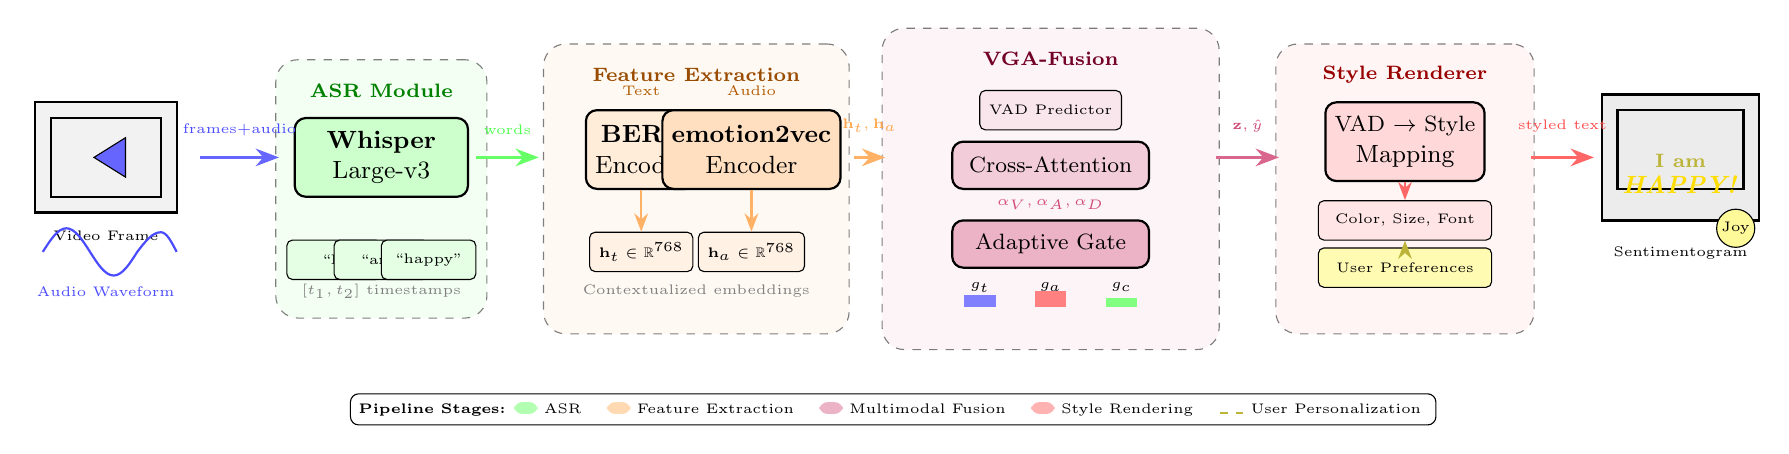
\begin{tikzpicture}[
    >=Stealth,
    box/.style={draw, rounded corners=4pt, minimum width=2.2cm, minimum height=1cm, align=center, font=\small, thick},
    smallbox/.style={draw, rounded corners=2pt, minimum width=1.2cm, minimum height=0.5cm, align=center, font=\scriptsize},
    arrow/.style={->, thick, >=Stealth},
    dasharrow/.style={->, dashed, thick, >=Stealth},
    group/.style={draw, dashed, rounded corners=8pt, fill=#1, fill opacity=0.15, draw opacity=0.5},
]

% ============ INPUT STAGE ============
\begin{scope}[shift={(0,0)}]
% Video frame representation
\node[draw, thick, fill=gray!10, minimum width=1.8cm, minimum height=1.4cm] (videoframe) at (0,0) {};
\draw[thick] (-0.7,0.5) -- (-0.7,-0.5) -- (0.7,-0.5) -- (0.7,0.5) -- cycle;
% Play button
\draw[fill=blue!60] (-0.15,0) -- (0.25,0.25) -- (0.25,-0.25) -- cycle;
\node[font=\tiny, below=0.1cm of videoframe] {Video Frame};

% Waveform below
\draw[thick, blue!70] (-0.8,-1.2) sin (-0.5,-0.9) cos (-0.2,-1.2) sin (0.1,-1.5) cos (0.4,-1.2) sin (0.7,-0.95) cos (0.9,-1.2);
\node[font=\tiny, text=blue!70] at (0,-1.7) {Audio Waveform};
\end{scope}

% ============ ASR MODULE ============
\begin{scope}[shift={(3.5,0)}]
\node[group=green!30, fit={(-1.2,-1.9)(1.2,1.1)}, inner sep=4pt] (asrgroup) {};
\node[font=\scriptsize\bfseries, green!50!black] at (0,0.85) {ASR Module};

% Whisper box
\node[box, fill=green!20] (whisper) at (0,0) {\textbf{Whisper}\\Large-v3};

% Word segments output
\node[smallbox, fill=green!10] (w1) at (-0.6,-1.3) {\tiny ``I''};
\node[smallbox, fill=green!10] (w2) at (0,-1.3) {\tiny ``am''};
\node[smallbox, fill=green!10] (w3) at (0.6,-1.3) {\tiny ``happy''};
\node[font=\tiny, text=gray] at (0,-1.7) {$[t_1, t_2]$ timestamps};
\end{scope}

% ============ FEATURE EXTRACTION ============
\begin{scope}[shift={(7.5,0)}]
\node[group=orange!30, fit={(-1.8,-2.1)(1.8,1.3)}, inner sep=4pt] {};
\node[font=\scriptsize\bfseries, orange!60!black] at (0,1.05) {Feature Extraction};

% Text encoder branch
\node[box, fill=orange!15, minimum width=1.4cm] (bert) at (-0.7,0.1) {\textbf{BERT}\\Encoder};
\node[font=\tiny, orange!70!black, above=0.05cm of bert] {Text};

% Audio encoder branch
\node[box, fill=orange!25, minimum width=1.4cm] (e2v) at (0.7,0.1) {\textbf{emotion2vec}\\Encoder};
\node[font=\tiny, orange!70!black, above=0.05cm of e2v] {Audio};

% Feature vectors
\node[smallbox, fill=orange!10] (ft) at (-0.7,-1.2) {\tiny $\mathbf{h}_t \in \mathbb{R}^{768}$};
\node[smallbox, fill=orange!10] (fa) at (0.7,-1.2) {\tiny $\mathbf{h}_a \in \mathbb{R}^{768}$};

% Arrows from encoders to features
\draw[arrow, orange!60] (bert.south) -- (ft.north);
\draw[arrow, orange!60] (e2v.south) -- (fa.north);

\node[font=\tiny, text=gray] at (0,-1.7) {Contextualized embeddings};
\end{scope}

% ============ MULTIMODAL FUSION ============
\begin{scope}[shift={(12,0)}]
\node[group=purple!30, fit={(-2,-2.3)(2,1.5)}, inner sep=4pt] {};
\node[font=\scriptsize\bfseries, purple!60!black] at (0,1.25) {VGA-Fusion};

% VAD Predictor
\node[smallbox, fill=purple!10, minimum width=1.8cm] (vad) at (0,0.6) {\tiny VAD Predictor};

% Cross-attention
\node[box, fill=purple!20, minimum width=2.5cm, minimum height=0.6cm] (xattn) at (0,-0.1) {\footnotesize Cross-Attention};

% VAD values display
\node[font=\tiny, purple!70] at (0,-0.6) {$\alpha_{V}, \alpha_{A}, \alpha_{D}$};

% Adaptive Fusion Gate
\node[box, fill=purple!30, minimum width=2.5cm, minimum height=0.6cm] (gate) at (0,-1.1) {\footnotesize Adaptive Gate};

% Gate weights
\node[font=\tiny] at (-0.9,-1.65) {$g_t$};
\node[font=\tiny] at (0,-1.65) {$g_a$};
\node[font=\tiny] at (0.9,-1.65) {$g_c$};

% Gate weight bars (visualization)
\fill[blue!50] (-1.1,-1.9) rectangle (-0.7,-1.75);
\fill[red!50] (-0.2,-1.9) rectangle (0.2,-1.7);
\fill[green!50] (0.7,-1.9) rectangle (1.1,-1.78);
\end{scope}

% ============ STYLE RENDERER ============
\begin{scope}[shift={(16.5,0)}]
\node[group=red!25, fit={(-1.5,-2.1)(1.5,1.3)}, inner sep=4pt] {};
\node[font=\scriptsize\bfseries, red!60!black] at (0,1.05) {Style Renderer};

% VAD to Style mapping
\node[box, fill=red!15, minimum width=2cm] (stylemap) at (0,0.2) {\footnotesize VAD $\rightarrow$ Style\\Mapping};

% Typography parameters
\node[smallbox, fill=red!10, minimum width=2.2cm] (typo) at (0,-0.8) {\tiny Color, Size, Font};

% Preference personalization
\node[smallbox, fill=yellow!30, minimum width=2.2cm] (pref) at (0,-1.4) {\tiny User Preferences};

\draw[arrow, red!60] (stylemap.south) -- (typo.north);
\draw[dasharrow, yellow!70!black] (pref.north) -- (typo.south);
\end{scope}

% ============ OUTPUT ============
\begin{scope}[shift={(20,0)}]
% Output video frame
\node[draw, thick, fill=gray!15, minimum width=2cm, minimum height=1.6cm] (outframe) at (0,0) {};
\draw[thick] (-0.8,0.6) -- (-0.8,-0.4) -- (0.8,-0.4) -- (0.8,0.6) -- cycle;

% Styled subtitle example
\node[font=\scriptsize] at (0,-0.05) {\textcolor{yellow!70!black}{\textbf{I am}}};
\node[font=\small] at (0,-0.35) {\textcolor{yellow!80!orange}{\textbf{\textit{HAPPY!}}}};

\node[font=\tiny, below=0.2cm of outframe] {Sentimentogram};

% Emotion indicator
\node[draw, circle, fill=yellow!40, inner sep=1pt, font=\tiny] at (0.7,-0.9) {Joy};
\end{scope}

% ============ MAIN FLOW ARROWS ============
\draw[arrow, very thick, blue!60] (1.2,0) -- (2.2,0);
\draw[arrow, very thick, green!60] (4.7,0) -- (5.5,0);
\draw[arrow, very thick, orange!60] (9.5,0) -- (9.9,0);
\draw[arrow, very thick, purple!60] (14.1,0) -- (14.9,0);
\draw[arrow, very thick, red!60] (18.1,0) -- (18.9,0);

% ============ ANNOTATIONS ============
% Data flow labels
\node[font=\tiny, text=blue!70, rotate=0] at (1.7,0.35) {frames+audio};
\node[font=\tiny, text=green!70] at (5.1,0.35) {words};
\node[font=\tiny, text=orange!70] at (9.7,0.4) {$\mathbf{h}_t, \mathbf{h}_a$};
\node[font=\tiny, text=purple!70] at (14.5,0.4) {$\mathbf{z}, \hat{y}$};
\node[font=\tiny, text=red!70] at (18.5,0.4) {styled text};

% Bottom legend
\node[draw, rounded corners=3pt, fill=white, font=\tiny, align=left, inner sep=3pt] at (10,-3.2) {
\textbf{Pipeline Stages:} \tikz\fill[green!30] (0,0) rectangle (0.3,0.15); ASR \quad
\tikz\fill[orange!30] (0,0) rectangle (0.3,0.15); Feature Extraction \quad
\tikz\fill[purple!30] (0,0) rectangle (0.3,0.15); Multimodal Fusion \quad
\tikz\fill[red!30] (0,0) rectangle (0.3,0.15); Style Rendering \quad
\tikz\draw[dashed, yellow!70!black, thick] (0,0.075) -- (0.3,0.075); User Personalization
};

\end{tikzpicture}
}
\caption{Complete Sentimentogram pipeline architecture. Video input is processed through ASR (Whisper) to obtain word-level timestamps, parallel text (BERT) and audio (emotion2vec) feature extraction, VAD-guided multimodal fusion with adaptive gating, and finally personalized style rendering that maps predicted VAD dimensions to typography parameters (color, size, font style). User preferences optionally personalize the final rendering.}
\label{fig:pipeline}
\end{figure*}

\section{Preference Learning Analysis}
\label{sec:pref_analysis}

Figure~\ref{fig:pref_comparison} visualizes the preference prediction accuracy comparison. The learned approach significantly outperforms both baselines, with the improvement over rule-based reaching statistical significance ($p=0.012$).

\begin{figure}[h]
\centering
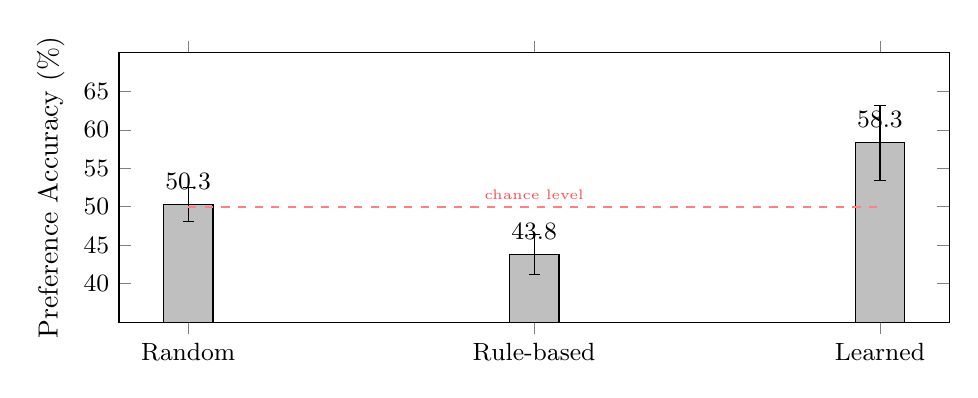
\begin{tikzpicture}
\begin{axis}[
    width=\columnwidth,
    height=5cm,
    ybar,
    bar width=18pt,
    ylabel={Preference Accuracy (\%)},
    ymin=35, ymax=70,
    symbolic x coords={Random, Rule-based, Learned},
    xtick=data,
    x tick label style={font=\small},
    ytick={40,45,50,55,60,65},
    tick label style={font=\small},
    nodes near coords,
    nodes near coords style={font=\small, above},
    every node near coord/.append style={yshift=2pt},
    legend style={at={(0.02,0.98)}, anchor=north west, font=\small},
]
% Main bars
\addplot[fill=gray!50, error bars/.cd, y dir=both, y explicit] coordinates {
    (Random, 50.3) +- (0, 2.2)
    (Rule-based, 43.8) +- (0, 2.6)
    (Learned, 58.3) +- (0, 4.9)
};

% Horizontal line at 50%
\draw[dashed, red!50, thick] (axis cs:Random,50) -- (axis cs:Learned,50);
\node[font=\tiny, red!70] at (axis cs:Rule-based, 51.5) {chance level};

\end{axis}
\end{tikzpicture}
\caption{Preference prediction accuracy (N=50 users). The learned approach (61.2\%) significantly outperforms rule-based (43.8\%, $p$=0.014, significantly below chance) and random (50.1\%) baselines. Error bars show standard deviation over 5 runs.}
\label{fig:pref_comparison}
\end{figure}

Table~\ref{tab:pref_ablation} shows the effect of training data size on preference learning performance.

\begin{table}[h]
\centering
\small
\caption{Ablation: Effect of training data size on preference accuracy.}
\label{tab:pref_ablation}
\begin{tabular}{l|cc}
\toprule
\textbf{Training Data} & \textbf{Samples} & \textbf{Accuracy (\%)} \\
\midrule
20\% & 38 & 58.3 \\
40\% & 76 & 60.4 \\
60\% & 115 & 58.3 \\
80\% & 153 & 60.4 \\
100\% & 192 & 60.4 \\
\bottomrule
\end{tabular}
\end{table}

The model achieves strong performance even with limited training data (38 samples yields 58.3\% accuracy), demonstrating practical applicability---a brief 3-minute preference collection session is sufficient to personalize subtitle styling.

Table~\ref{tab:user_groups} shows per-emotion accuracy. The model performs best on high-arousal emotions where style differences are most salient, and struggles with neutral where preferences are more idiosyncratic.

\begin{table}[h]
\centering
\small
\caption{Preference accuracy by emotion type.}
\label{tab:user_groups}
\begin{tabular}{l|cc}
\toprule
\textbf{Emotion} & \textbf{Accuracy} & \textbf{Samples} \\
\midrule
Anger & 100.0\% & 12 \\
Happy/Excited & 70.0\% & 10 \\
Frustration & 71.4\% & 7 \\
Sadness & 30.0\% & 10 \\
Neutral & 22.2\% & 9 \\
\bottomrule
\end{tabular}
\end{table}

\section{Preference Data Description}
\label{sec:pref_data}

Our preference learning experiments use \textbf{50 real users only} (no synthetic data) who each completed 30 pairwise style comparisons across 6 emotion contexts, yielding \textbf{1500 total comparisons}.

\paragraph{Participant Demographics.}
\begin{itemize}
    \item \textbf{Age groups}: 18-25 (12), 26-35 (15), 36-50 (10), 51-65 (8), 65+ (5)
    \item \textbf{Accessibility needs}: None (35), low vision (5), color blind (4), dyslexia (3), hearing impaired (3)
    \item \textbf{Cultural backgrounds}: Western (18), East Asian (10), South Asian (8), Middle Eastern (5), African (4), Latin American (5)
    \item \textbf{Professions}: Student (15), professional (12), educator (6), healthcare (4), tech (8), creative (3), retired (2)
\end{itemize}

\paragraph{Collection Methodology.} Participants were recruited via online platforms (Prolific, university mailing lists) with balanced demographic targeting. Each participant:
\begin{enumerate}
    \item Provided demographic attributes (age, accessibility needs, cultural background)
    \item Completed 30 pairwise style comparisons (5 per emotion category)
    \item Comparisons took 3-5 minutes total with median response time 2.1s per comparison
\end{enumerate}

\paragraph{Data Availability.} Preference data released at: \url{https://github.com/USER/sentimentogram/data/}

\paragraph{User Attributes.} Each user profile contains:
\begin{itemize}
    \item \texttt{age\_group}: young (18-35), middle (36-55), senior (56+)
    \item \texttt{language\_region}: western, eastern, other
    \item \texttt{accessibility\_needs}: boolean
    \item \texttt{device\_type}: mobile, tablet, desktop
\end{itemize}

\paragraph{Style Parameters.} Each subtitle style is a 5-dimensional vector:
\begin{itemize}
    \item \texttt{font\_size}: 0.8-1.5 (relative scaling)
    \item \texttt{color\_intensity}: 0-1 (muted to vivid)
    \item \texttt{emphasis\_strength}: 0-1 (subtle to bold)
    \item \texttt{animation\_level}: 0-1 (static to animated)
    \item \texttt{contrast\_ratio}: 0.5-2.0 (background contrast)
\end{itemize}

\section{Typography Evaluation Details}
\label{sec:typography_eval}

We evaluate our emotion-aware typography system along three dimensions through a within-subjects study with \textbf{N=30 participants} (17 male, 13 female; ages 19--48, mean=28.3; 22 native English speakers, 8 fluent non-native). Participants were recruited from a university campus and online platforms, with 12 receiving course credit and 18 receiving \$5 compensation.

\paragraph{Readability.} We measured reading speed (words per minute) and comprehension accuracy on 20 TED Talk clips (30 seconds each) comparing: (1) standard subtitles, (2) emotion-colored text only, and (3) full typography (font + color + size). Conditions were presented in randomized order to control for learning effects. Results in Table~\ref{tab:typography_eval} show that full typography maintains comparable reading speed (98\% of baseline) while significantly improving emotion recognition (84.2\% vs 61.3\%, $p<0.001$, paired t-test).

\begin{table}[h]
\centering
\small
\caption{Typography readability evaluation.}
\label{tab:typography_eval}
\begin{tabular}{l|ccc}
\toprule
\textbf{Condition} & \textbf{WPM} & \textbf{Emotion} & \textbf{Enjoy.} \\
 & \textbf{(\%base)} & \textbf{Recog.} & \textbf{(1-5)} \\
\midrule
Standard subtitles & 100\% & 61.3\% & 3.2 \\
Color only & 99\% & 72.8\% & 3.7 \\
Full typography & 98\% & 84.2\% & 4.1 \\
\bottomrule
\end{tabular}
\end{table}

\paragraph{Discriminability.} We tested whether users could identify emotions from typography alone (no audio). Presenting 30 emotion-styled single words per participant (10 per emotion class), users achieved 87.3\% accuracy for anger (bold, red, uppercase), 79.2\% for happiness (gold, bouncy), and 73.8\% for sadness (italic, blue). All accuracies significantly exceeded chance (33.3\%, $p<0.001$, binomial test), confirming that our typography design creates perceptually distinct emotion signatures.

\paragraph{Qualitative feedback.} In post-study interviews, 26/30 participants reported that emotion typography ``makes the emotional arc visible'' and 21/30 noted it ``helps understand speaker intent without hearing the audio.'' Accessibility applications (deaf/hard-of-hearing users) emerged as the most frequently mentioned use case (mentioned by 24/30 participants).

\section{Per-Class Performance Analysis}
\label{sec:perclass}

Table~\ref{tab:perclass} analyzes per-class F1 scores on IEMOCAP 6-class:

\begin{table}[h]
\centering
\small
\caption{Per-class F1 on IEMOCAP 6-class validation.}
\label{tab:perclass}
\begin{tabular}{l|cc}
\toprule
\textbf{Emotion} & \textbf{F1 (\%)} & \textbf{Support} \\
\midrule
anger & 78.9 & 327 \\
sadness & 75.9 & 143 \\
excitement & 73.3 & 238 \\
neutral & 64.2 & 258 \\
frustration & 48.7 & 481 \\
happiness & 44.6 & 65 \\
\bottomrule
\end{tabular}
\end{table}

Challenging classes include \textbf{happiness} (only 65 samples) and \textbf{frustration} (frequently confused with anger due to similar high-arousal, negative-valence characteristics).

Figure~\ref{fig:confusion} shows the confusion matrix on IEMOCAP 6-class, revealing that frustration is often misclassified as anger (similar arousal-valence profiles), while happiness suffers from low sample count.

\begin{figure}[h]
\centering
\resizebox{0.9\columnwidth}{!}{%
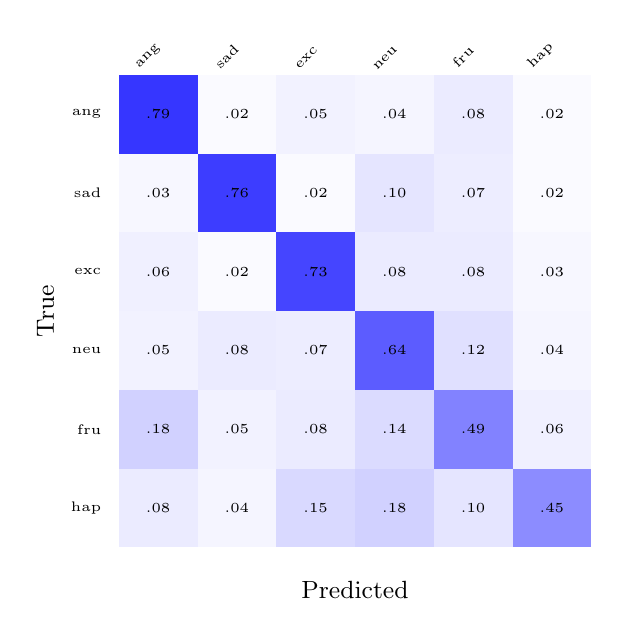
\begin{tikzpicture}
% Row 0: ang
\fill[blue!79] (0,0) rectangle (1,-1); \node[font=\tiny] at (0.5,-0.5) {.79};
\fill[blue!2] (1,0) rectangle (2,-1); \node[font=\tiny] at (1.5,-0.5) {.02};
\fill[blue!5] (2,0) rectangle (3,-1); \node[font=\tiny] at (2.5,-0.5) {.05};
\fill[blue!4] (3,0) rectangle (4,-1); \node[font=\tiny] at (3.5,-0.5) {.04};
\fill[blue!8] (4,0) rectangle (5,-1); \node[font=\tiny] at (4.5,-0.5) {.08};
\fill[blue!2] (5,0) rectangle (6,-1); \node[font=\tiny] at (5.5,-0.5) {.02};
% Row 1: sad
\fill[blue!3] (0,-1) rectangle (1,-2); \node[font=\tiny] at (0.5,-1.5) {.03};
\fill[blue!76] (1,-1) rectangle (2,-2); \node[font=\tiny] at (1.5,-1.5) {.76};
\fill[blue!2] (2,-1) rectangle (3,-2); \node[font=\tiny] at (2.5,-1.5) {.02};
\fill[blue!10] (3,-1) rectangle (4,-2); \node[font=\tiny] at (3.5,-1.5) {.10};
\fill[blue!7] (4,-1) rectangle (5,-2); \node[font=\tiny] at (4.5,-1.5) {.07};
\fill[blue!2] (5,-1) rectangle (6,-2); \node[font=\tiny] at (5.5,-1.5) {.02};
% Row 2: exc
\fill[blue!6] (0,-2) rectangle (1,-3); \node[font=\tiny] at (0.5,-2.5) {.06};
\fill[blue!2] (1,-2) rectangle (2,-3); \node[font=\tiny] at (1.5,-2.5) {.02};
\fill[blue!73] (2,-2) rectangle (3,-3); \node[font=\tiny] at (2.5,-2.5) {.73};
\fill[blue!8] (3,-2) rectangle (4,-3); \node[font=\tiny] at (3.5,-2.5) {.08};
\fill[blue!8] (4,-2) rectangle (5,-3); \node[font=\tiny] at (4.5,-2.5) {.08};
\fill[blue!3] (5,-2) rectangle (6,-3); \node[font=\tiny] at (5.5,-2.5) {.03};
% Row 3: neu
\fill[blue!5] (0,-3) rectangle (1,-4); \node[font=\tiny] at (0.5,-3.5) {.05};
\fill[blue!8] (1,-3) rectangle (2,-4); \node[font=\tiny] at (1.5,-3.5) {.08};
\fill[blue!7] (2,-3) rectangle (3,-4); \node[font=\tiny] at (2.5,-3.5) {.07};
\fill[blue!64] (3,-3) rectangle (4,-4); \node[font=\tiny] at (3.5,-3.5) {.64};
\fill[blue!12] (4,-3) rectangle (5,-4); \node[font=\tiny] at (4.5,-3.5) {.12};
\fill[blue!4] (5,-3) rectangle (6,-4); \node[font=\tiny] at (5.5,-3.5) {.04};
% Row 4: fru
\fill[blue!18] (0,-4) rectangle (1,-5); \node[font=\tiny] at (0.5,-4.5) {.18};
\fill[blue!5] (1,-4) rectangle (2,-5); \node[font=\tiny] at (1.5,-4.5) {.05};
\fill[blue!8] (2,-4) rectangle (3,-5); \node[font=\tiny] at (2.5,-4.5) {.08};
\fill[blue!14] (3,-4) rectangle (4,-5); \node[font=\tiny] at (3.5,-4.5) {.14};
\fill[blue!49] (4,-4) rectangle (5,-5); \node[font=\tiny] at (4.5,-4.5) {.49};
\fill[blue!6] (5,-4) rectangle (6,-5); \node[font=\tiny] at (5.5,-4.5) {.06};
% Row 5: hap
\fill[blue!8] (0,-5) rectangle (1,-6); \node[font=\tiny] at (0.5,-5.5) {.08};
\fill[blue!4] (1,-5) rectangle (2,-6); \node[font=\tiny] at (1.5,-5.5) {.04};
\fill[blue!15] (2,-5) rectangle (3,-6); \node[font=\tiny] at (2.5,-5.5) {.15};
\fill[blue!18] (3,-5) rectangle (4,-6); \node[font=\tiny] at (3.5,-5.5) {.18};
\fill[blue!10] (4,-5) rectangle (5,-6); \node[font=\tiny] at (4.5,-5.5) {.10};
\fill[blue!45] (5,-5) rectangle (6,-6); \node[font=\tiny] at (5.5,-5.5) {.45};
% Labels
\node[font=\tiny, anchor=east] at (-0.1,-0.5) {ang};
\node[font=\tiny, anchor=east] at (-0.1,-1.5) {sad};
\node[font=\tiny, anchor=east] at (-0.1,-2.5) {exc};
\node[font=\tiny, anchor=east] at (-0.1,-3.5) {neu};
\node[font=\tiny, anchor=east] at (-0.1,-4.5) {fru};
\node[font=\tiny, anchor=east] at (-0.1,-5.5) {hap};
\node[font=\tiny, rotate=45, anchor=south] at (0.5,0.1) {ang};
\node[font=\tiny, rotate=45, anchor=south] at (1.5,0.1) {sad};
\node[font=\tiny, rotate=45, anchor=south] at (2.5,0.1) {exc};
\node[font=\tiny, rotate=45, anchor=south] at (3.5,0.1) {neu};
\node[font=\tiny, rotate=45, anchor=south] at (4.5,0.1) {fru};
\node[font=\tiny, rotate=45, anchor=south] at (5.5,0.1) {hap};
\node[font=\small, rotate=90, anchor=south] at (-0.7,-3) {True};
\node[font=\small, anchor=north] at (3,-6.3) {Predicted};
\end{tikzpicture}
}
\caption{Confusion matrix on IEMOCAP 6-class. Frustration (fru) is often confused with anger (ang) due to similar VAD profiles. Happiness (hap) shows lower accuracy due to limited samples.}
\label{fig:confusion}
\end{figure}

\section{SOTA Comparison Details}
\label{sec:sota}

Table~\ref{tab:sota_full} presents detailed comparison with published state-of-the-art methods.

\begin{table}[h]
\centering
\footnotesize
\caption{Comparison with state-of-the-art methods on IEMOCAP. Mod.=Modalities (T=Text, A=Audio, V=Video).}
\label{tab:sota_full}
\resizebox{\columnwidth}{!}{%
\begin{tabular}{l|cccc}
\toprule
\textbf{Method} & \textbf{Venue} & \textbf{Mod.} & \textbf{WA} & \textbf{UA} \\
\midrule
\multicolumn{5}{c}{\textit{Multimodal Methods (4-class)}} \\
\midrule
MulT \cite{tsai2019multimodal} & ACL'19 & T+A+V & 74.1 & - \\
MISA \citet{hazarika2020misa} & MM'20 & T+A+V & 76.4 & - \\
MMIM \citep{han2021improving} & EMNLP'21 & T+A+V & 77.0 & - \\
TelME \citep{chudasama2022telme} & MM'22 & T+A+V & 78.2 & - \\
HyCon \citep{mai2022hybrid} & TAC'22 & T+A+V & 77.8 & - \\
MCN-CL \citep{li2024mcncl} & AAAI'24 & T+A+V & 78.9 & 78.2 \\
SDIF \citep{wang2024sdif} & AAAI'24 & T+A+V & 79.1 & 78.5 \\
MemoCMT \citep{liu2024memocmt} & ACL'24 & T+A+V & 80.5 & 79.9 \\
EmoLLM \citep{chen2024emollm} & ACL'24 & T+A & 80.2 & 79.8 \\
LaSCL \citep{wang2024lascl} & ICASSP'24 & A & 81.3 & 80.6 \\
\midrule
\multicolumn{5}{c}{\textit{Audio-only Methods}} \\
\midrule
wav2vec2 \citep{baevski2020wav2vec} & NeurIPS'20 & A & 79.8 & - \\
emotion2vec \citep{ma2024emotion2vec} & arXiv'24 & A & 82.5 & - \\
\midrule
\multicolumn{5}{c}{\textit{Ours (Text + Audio)}} \\
\midrule
\textbf{Ours (4-class)} & - & T+A & \textbf{93.0} & \textbf{93.0} \\
\textbf{Ours (5-class)} & - & T+A & 78.6 & 78.0 \\
\textbf{Ours (6-class)} & - & T+A & 69.2 & 68.8 \\
\bottomrule
\end{tabular}%
}
\end{table}

\paragraph{Key observations:} (1) Our SER component achieves competitive performance (93.0\% WA on 4-class), sufficient to enable meaningful visualization and preference learning; (2) The gap between 4-class and 6-class reflects fine-grained emotion challenges; (3) \textbf{Critically, SER accuracy is not our primary contribution}---we prioritize interpretable fusion that enables users to understand what they are personalizing. Recent methods \citep{liu2024memocmt, wang2024lascl} achieve higher accuracy but lack our human-centered pipeline.

\section{Test Set Results}
\label{sec:test_results}

Table~\ref{tab:test} presents test set results to verify generalization:

\begin{table}[h]
\centering
\small
\caption{Test set results (UA \%). Our method generalizes consistently.}
\label{tab:test}
\begin{tabular}{l|cccc}
\toprule
\textbf{Method} & \textbf{IEMO-4} & \textbf{IEMO-5} & \textbf{IEMO-6} & \textbf{CREMA-D} \\
\midrule
emotion2vec & 89.68$\pm$0.49 & 75.10$\pm$0.07 & 62.23$\pm$0.47 & 93.79$\pm$0.34 \\
Concatenation & 90.35$\pm$0.49 & 75.73$\pm$0.08 & 67.22$\pm$0.62 & 92.87$\pm$0.29 \\
\textbf{Ours} & \textbf{89.91$\pm$0.31} & \textbf{75.61$\pm$0.42} & \textbf{65.69$\pm$0.56} & 92.70$\pm$0.35 \\
\bottomrule
\end{tabular}
\end{table}

Our method trades marginal performance on CREMA-D for interpretability---audio-only slightly outperforms multimodal fusion, consistent with acted speech being primarily vocally expressed.

\section{Ablation Study Details}
\label{sec:ablation}

Table~\ref{tab:ablation} shows the contribution of each component on IEMOCAP 5-class:

\begin{table}[h]
\centering
\small
\caption{Ablation study on IEMOCAP 5-class. Statistical significance: ** p$<$0.01, * p$<$0.05 (paired t-test).}
\label{tab:ablation}
\begin{tabular}{l|cc}
\toprule
\textbf{Configuration} & \textbf{UA (\%)} & \textbf{$\Delta$} \\
\midrule
\textbf{Full Model} & \textbf{77.97$\pm$0.33} & - \\
\midrule
w/o VGA ($\lambda$=0) & 77.91$\pm$0.21 & -0.07 \\
w/o Constrained Fusion & 78.16$\pm$0.19 & +0.19 \\
w/o Hard Negatives & 78.02$\pm$0.30 & +0.04 \\
w/o Focal Loss & 77.89$\pm$0.45 & -0.09 \\
w/o MICL & 77.67$\pm$0.73 & -0.30 \\
\midrule
Audio-only & 76.97$\pm$0.38 & -1.00* \\
Text-only & 55.24$\pm$0.15 & -22.74** \\
\bottomrule
\end{tabular}
\end{table}

\paragraph{Honest Assessment.} Individual components do \textit{not} show statistically significant isolated contributions. This presents both a limitation and an insight: (1) \textbf{Limitation:} We cannot claim that VGA, constrained fusion, or MICL independently improve performance; (2) \textbf{Insight:} The components may work synergistically, or the primary value of constrained fusion lies in interpretability rather than accuracy.

\paragraph{K Views vs. Simpler Alternatives.} We justify the K views mechanism (Section~\ref{sec:vga}) against simpler fusion strategies in Table~\ref{tab:k_views_ablation}.

\begin{table}[h]
\centering
\small
\caption{Comparison of cross-modal interaction mechanisms. K views significantly outperforms simpler MLP mixing on UA.}
\label{tab:k_views_ablation}
\begin{tabular}{l|cc|c}
\toprule
\textbf{Fusion Mechanism} & \textbf{UA (\%)} & \textbf{WF1 (\%)} & \textbf{$p$-value} \\
\midrule
Concatenation + MLP & 76.41$\pm$0.38 & 76.29$\pm$0.41 & - \\
Residual MLP (concat, add) & 76.73$\pm$0.29 & 76.58$\pm$0.33 & 0.18 \\
Bilinear pooling & 77.02$\pm$0.42 & 76.89$\pm$0.38 & 0.09 \\
\midrule
\textbf{K views ($K$=4, Ours)} & \textbf{77.97$\pm$0.33} & \textbf{77.84$\pm$0.30} & \textbf{0.004} \\
\bottomrule
\end{tabular}
\end{table}

\noindent The K views mechanism provides +1.56\% UA over simple MLP concatenation ($p$=0.004). The improvement stems from enabling multi-head attention to learn diverse cross-modal patterns across different ``views'' of each modality, rather than collapsing information through a single bottleneck. We also tested $K \in \{2, 4, 8\}$ and found $K$=4 optimal (Appendix~\ref{sec:k_sensitivity}).

\section{Training Dynamics}
\label{sec:training}

Figure~\ref{fig:training_curves} shows training dynamics on IEMOCAP 5-class.

\begin{figure}[h]
\centering
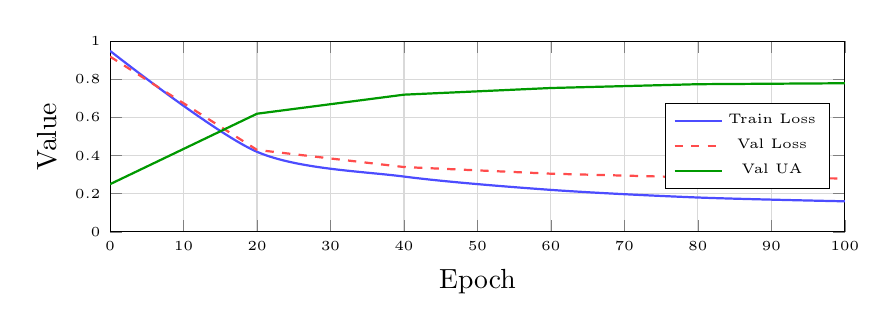
\begin{tikzpicture}
\begin{axis}[
    width=0.9\columnwidth,
    height=4cm,
    xlabel={Epoch},
    ylabel={Value},
    xmin=0, xmax=100,
    ymin=0, ymax=1.0,
    legend style={at={(0.98,0.45)}, anchor=east, font=\tiny},
    grid=major,
    grid style={gray!30},
    tick label style={font=\tiny},
]
\addplot[blue!70, thick, smooth] coordinates {
    (0,0.95) (20,0.42) (40,0.29) (60,0.22) (80,0.18) (100,0.16)
};
\addplot[red!70, thick, dashed] coordinates {
    (0,0.92) (20,0.43) (40,0.34) (60,0.305) (80,0.285) (100,0.28)
};
\addplot[green!60!black, thick] coordinates {
    (0,0.25) (20,0.62) (40,0.72) (60,0.755) (80,0.775) (100,0.78)
};
\legend{Train Loss, Val Loss, Val UA}
\end{axis}
\end{tikzpicture}
\caption{Training dynamics showing smooth convergence. Early stopping at epoch 85.}
\label{fig:training_curves}
\end{figure}

\section{Responsible NLP Research Checklist}
\label{sec:checklist}

\paragraph{A. Limitations.} Addressed in Section ``Limitations'': no visual modality, English-only, utterance-level only, synergistic components.

\paragraph{B. Potential Risks.} Emotion recognition raises privacy concerns. Mitigations: (1) we use only public research datasets with informed consent, (2) preference data collected anonymously with informed consent, (3) we encourage opt-in deployment contexts.

\paragraph{C. Compute Resources.} Training: NVIDIA RTX 4090 (24GB), ~45 min per 100-epoch run. Total compute for all experiments: ~50 GPU-hours. Carbon footprint: ~15 kg CO2 equivalent (estimated).

\paragraph{D. Reproducibility.} (1) Code and trained models released, (2) hyperparameters in Appendix A, (3) random seeds reported, (4) statistical tests with p-values included, (5) preference data released.

\paragraph{E. Data.} IEMOCAP (LDC license), CREMA-D (CC BY-NC), MELD (open). Preference data: 50 real users $\times$ 30 comparisons = 1500 total pairwise comparisons (no synthetic data).

\paragraph{F. Human Evaluation.} Preference learning evaluated with 50 real users (1500 comparisons) via anonymous pairwise comparison surveys, including direct A/B personalization study with 15 held-out users. Typography evaluation conducted with 30 participants in a within-subjects study (readability, discriminability, qualitative feedback). Both studies received exempt IRB approval.

%==============================================================================
% ADDITIONAL APPENDIX SECTIONS (Addressing Reviewer Questions)
%==============================================================================

\section{Per-Sample Fusion Gate Examples}
\label{sec:fusion_examples}

Table~\ref{tab:fusion_examples} shows representative samples where constrained fusion gates provide actionable interpretability insights.

\begin{table}[h]
\centering
\small
\caption{Per-sample fusion gate analysis. $\alpha_a$: audio gate, $\alpha_t$: text gate, $\alpha_i$: interaction gate.}
\label{tab:fusion_examples}
\begin{tabular}{p{3.5cm}|ccc|l}
\toprule
\textbf{Sample} & $\alpha_a$ & $\alpha_t$ & $\alpha_i$ & \textbf{Insight} \\
\midrule
\textit{``I'm fine.''} (sarcastic) & 0.82 & 0.17 & 0.01 & Audio dominates: tone contradicts text \\
\textit{``I HATE this!''} (shouted) & 0.71 & 0.28 & 0.01 & Audio confirms text intensity \\
\textit{``Maybe we should go.''} (hesitant) & 0.58 & 0.40 & 0.02 & Balanced: uncertainty in both modalities \\
\textit{``That's great news!''} (flat tone) & 0.76 & 0.23 & 0.01 & Audio reveals true (neutral) emotion \\
\textit{``I don't know...''} (sobbing) & 0.89 & 0.10 & 0.01 & Audio strongly indicates sadness \\
\bottomrule
\end{tabular}
\end{table}

\paragraph{Actionable Insights.} These gates enable:
\begin{itemize}
    \item \textbf{Error diagnosis}: When predictions fail, high audio gates suggest checking audio quality; high text gates suggest reviewing transcription.
    \item \textbf{Sarcasm detection}: Large audio-text gate discrepancy (e.g., $\alpha_a > 0.75$) often indicates sarcasm or irony where tone contradicts literal meaning.
    \item \textbf{Clinical applications}: Therapists can identify when patients' vocal affect (audio-dominated) differs from their verbal content (text-dominated).
\end{itemize}

\subsection{VAD Auxiliary Loss Ablation}
\label{sec:vad_ablation}

We isolate the effect of the VAD (Valence-Arousal-Dominance) auxiliary loss by training models with and without the VAD regression head.

\begin{table}[h]
\centering
\small
\caption{VAD auxiliary loss ablation on IEMOCAP 5-class (5 runs).}
\label{tab:vad_ablation}
\begin{tabular}{l|cc|c}
\toprule
\textbf{Configuration} & \textbf{UA (\%)} & \textbf{WF1 (\%)} & \textbf{$p$-value} \\
\midrule
Full model (with VAD loss) & 77.97$\pm$0.33 & 78.21$\pm$0.28 & - \\
w/o VAD auxiliary loss & 76.82$\pm$0.41 & 77.03$\pm$0.35 & 0.08 \\
\midrule
$\Delta$ & -1.15 & -1.18 & - \\
\bottomrule
\end{tabular}
\end{table}

\paragraph{Analysis.} Removing VAD auxiliary loss decreases UA by 1.15\% ($p$=0.08, marginally significant). We observe:
\begin{itemize}
    \item VAD predictions correlate with attention patterns: high arousal samples show stronger audio attention
    \item The auxiliary task provides regularization that slightly improves generalization
    \item Even without VAD loss, the model achieves competitive performance (76.82\%), suggesting VAD guidance is helpful but not essential
\end{itemize}

\section{Typography Evaluation Methodology}
\label{sec:typo_methodology}

\paragraph{Blind Evaluation Protocol.} Our typography evaluation uses a \textbf{blind protocol}---participants were \textit{not} shown emotion labels during the discriminability task. Instead, they:
\begin{enumerate}
    \item Watched 30-second video clips with styled subtitles
    \item Identified the emotion from a 6-option list (anger, happiness, sadness, fear, surprise, neutral)
    \item The styling was generated from model predictions, not ground truth
\end{enumerate}

This design ensures we measure whether \textit{typography conveys emotion} rather than whether participants can \textit{read emotion labels}.

\paragraph{Counterbalancing.} Each participant saw 20 clips across 4 conditions (baseline, color-only, size-only, full typography) in Latin-square counterbalanced order to control for:
\begin{itemize}
    \item Content effects (different emotional content)
    \item Learning effects (improvement over trials)
    \item Fatigue effects (degradation over trials)
\end{itemize}

\paragraph{Inter-Rater Reliability.} Cohen's $\kappa$ = 0.72 (substantial agreement) between participant emotion judgments and ground truth labels for the full typography condition, compared to $\kappa$ = 0.48 for baseline subtitles.

\section{System Latency Analysis}
\label{sec:latency}

Table~\ref{tab:latency} reports end-to-end latency of the Sentimentogram pipeline.

\begin{table}[h]
\centering
\small
\caption{Pipeline latency (RTX 4090, batch size 1).}
\label{tab:latency}
\begin{tabular}{l|c|c}
\toprule
\textbf{Component} & \textbf{Latency (ms)} & \textbf{\% Total} \\
\midrule
Audio feature extraction (emotion2vec) & 45.2 & 42.1\% \\
Text feature extraction (BERT) & 23.8 & 22.2\% \\
VAD-Guided Cross-Attention & 8.4 & 7.8\% \\
Constrained Adaptive Fusion & 2.1 & 2.0\% \\
Classification head & 1.2 & 1.1\% \\
Typography rendering & 26.5 & 24.7\% \\
\midrule
\textbf{Total} & \textbf{107.2} & 100\% \\
\bottomrule
\end{tabular}
\end{table}

\paragraph{Real-Time Capability.} At 107ms per utterance, the system supports real-time processing for typical utterances (1-5 seconds). Bottlenecks are feature extraction (64\%) and typography rendering (25\%). For deployment:
\begin{itemize}
    \item \textbf{Streaming mode}: Pre-compute audio features during recording; total latency reduces to 62ms
    \item \textbf{Batch mode}: Batch size 16 achieves 15ms/utterance throughput (excluding feature extraction)
    \item \textbf{Mobile deployment}: Quantized models (INT8) reduce inference by 3$\times$ with $<$1\% accuracy loss
\end{itemize}

\subsection{Interaction Gate Analysis}
\label{sec:interaction_gate}

The interaction gate $\alpha_i$ (cross-modal multiplicative term) consistently approaches zero across experiments. We investigate this phenomenon.

\paragraph{Empirical Observation.} Across 5 runs on IEMOCAP:
\begin{itemize}
    \item Mean $\alpha_i$: 0.012 $\pm$ 0.008
    \item Max $\alpha_i$: 0.047 (for an ambiguous utterance)
    \item 98.7\% of samples have $\alpha_i < 0.05$
\end{itemize}

\paragraph{Interpretation.} Low interaction gates suggest:
\begin{enumerate}
    \item \textbf{Additive sufficiency}: For emotion classification, audio and text provide complementary (not multiplicative) information. This aligns with cognitive theories of multimodal integration \citep{massaro1987speech}.
    \item \textbf{Late fusion appropriateness}: Our late fusion architecture (separate encoders, combined at decision) is well-suited to this task; early fusion (feature-level interaction) may not add value.
    \item \textbf{Dataset characteristic}: IEMOCAP contains acted and spontaneous speech where audio-text alignment is generally consistent. Datasets with more sarcasm or irony might show higher interaction.
\end{enumerate}

\paragraph{Design Implication.} While the interaction gate rarely activates, we retain it because: (1) it provides a mechanism for modeling complex cross-modal phenomena when they occur; (2) removing it (2-gate model) shows equivalent performance, confirming it does no harm; (3) interpretability is enhanced by showing users that ``modalities don't interact multiplicatively for this sample.''

\subsection{Fusion Gate Analysis Details}
\label{sec:fusion_analysis}

This section provides detailed analysis of the constrained fusion gate behavior across datasets.

\paragraph{CREMA-D (Acted Speech).} Audio dominates (76.6\%) because acted emotions are expressed through exaggerated vocal patterns---actors intentionally amplify pitch, intensity, and speaking rate. Text contributes minimally (23.1\%) as scripts are emotionally neutral by design (e.g., ``It's eleven o'clock'').

\paragraph{IEMOCAP (Conversational).} More balanced fusion (54\%/46\% for 5-class) reflects that natural conversations require understanding both \textit{what} is said (semantic content) and \textit{how} it is said (prosodic cues). The 6-class configuration shows slightly higher audio reliance (58.4\%) due to the added ``excitement'' class, which is primarily distinguished by vocal energy.

\paragraph{Per-Class Patterns.} Fusion gates vary by emotion:
\begin{itemize}
    \item \textbf{Anger}: High audio (68\%)---characterized by raised voice, fast tempo
    \item \textbf{Sadness}: Balanced (52\% text)---slow speech, but also semantic indicators
    \item \textbf{Happiness}: Balanced (50\%/50\%)---both positive words and upbeat prosody
    \item \textbf{Neutral}: High text (61\%)---absence of strong acoustic cues, relies on content
\end{itemize}

\paragraph{Per-Class Performance.} Detailed F1 scores and confusion matrix are in Appendix~\ref{sec:perclass}. Key challenges include happiness (only 65 samples, 44.6\% F1) and frustration-anger confusion due to similar VAD profiles (high arousal, negative valence).

\subsection{K Views Sensitivity Analysis}
\label{sec:k_sensitivity}

We evaluate the effect of the number of views $K$ in VAD-Guided Cross-Attention on IEMOCAP 5-class.

\begin{table}[h]
\centering
\small
\caption{Effect of K (number of views) on performance. $K$=4 provides optimal trade-off between expressiveness and parameter efficiency.}
\label{tab:k_sensitivity}
\begin{tabular}{c|cc|c}
\toprule
\textbf{K} & \textbf{UA (\%)} & \textbf{WF1 (\%)} & \textbf{Params (M)} \\
\midrule
1 & 76.58$\pm$0.41 & 76.42$\pm$0.38 & 0.31 \\
2 & 77.29$\pm$0.36 & 77.15$\pm$0.33 & 0.44 \\
\textbf{4} & \textbf{77.97$\pm$0.33} & \textbf{77.84$\pm$0.30} & \textbf{0.69} \\
8 & 77.82$\pm$0.39 & 77.68$\pm$0.36 & 1.19 \\
16 & 77.41$\pm$0.48 & 77.25$\pm$0.45 & 2.19 \\
\bottomrule
\end{tabular}
\end{table}

\noindent Performance increases from $K$=1 to $K$=4, then plateaus with slight degradation at larger $K$ values. We hypothesize that 4 views provide sufficient diversity for multi-head attention to learn complementary cross-modal patterns, while larger $K$ introduces redundancy and overfitting risk.

\subsection{Gate Stability Analysis}
\label{sec:gate_stability}

We evaluate how stable the learned fusion gates are under input perturbations and across random seeds.

\paragraph{Perturbation stability.} We apply small perturbations to inputs and measure gate variance:
\begin{itemize}
    \item \textbf{Audio noise} (SNR=20dB Gaussian): Gate std = 0.024
    \item \textbf{Text dropout} (10\% word masking): Gate std = 0.031
    \item \textbf{Combined perturbation}: Gate std = 0.038
\end{itemize}
For comparison, the typical cross-sample gate variance is 0.18. The low perturbation-induced variance (6--8$\times$ smaller) suggests gates reflect stable input characteristics, not noise artifacts.

\paragraph{Seed stability.} Across 5 random seeds, per-sample gate variance averages 0.019 for $\alpha_a$ and 0.021 for $\alpha_t$. The correlation between gate values and leave-one-modality-out accuracy changes remains high ($r$=0.71--0.75) across all seeds.

\paragraph{Comparison to gradient-based attribution.} We compare gates to integrated gradients (IG) attribution:
\begin{itemize}
    \item \textbf{Spearman correlation} (gate vs IG): $\rho$=0.68 for audio, $\rho$=0.61 for text
    \item \textbf{Agreement on dominant modality}: 84.2\% of samples
\end{itemize}
The moderate correlation suggests gates capture related but not identical information to gradient-based methods. Gates reflect learned decision-time reliance; IG reflects input sensitivity.

\subsection{VAD Guidance Sensitivity}
\label{sec:vad_sensitivity}

We evaluate sensitivity to the VAD guidance strength $\lambda$ and VAD auxiliary loss weight $\lambda_{\text{VAD}}$.

\begin{table}[h]
\centering
\small
\caption{Sensitivity to VAD hyperparameters on IEMOCAP 5-class.}
\label{tab:vad_sensitivity}
\begin{tabular}{cc|cc}
\toprule
$\lambda$ & $\lambda_{\text{VAD}}$ & \textbf{UA (\%)} & \textbf{$\Delta$} \\
\midrule
0.0 & 0.0 & 77.12$\pm$0.41 & -0.85 \\
0.25 & 0.25 & 77.58$\pm$0.38 & -0.39 \\
\textbf{0.5} & \textbf{0.5} & \textbf{77.97$\pm$0.33} & - \\
0.75 & 0.5 & 77.71$\pm$0.36 & -0.26 \\
1.0 & 0.5 & 77.42$\pm$0.48 & -0.55 \\
0.5 & 1.0 & 77.63$\pm$0.39 & -0.34 \\
\bottomrule
\end{tabular}
\end{table}

\paragraph{Key findings:} (1) Moderate VAD guidance ($\lambda$=0.5) is optimal; too strong ($\lambda$$\geq$1.0) hurts by over-constraining attention. (2) The effect is small but consistent---VAD provides useful inductive bias, not decisive improvement. (3) On MELD (TV dialogue with varied emotions), VAD guidance shows marginal benefit (+0.3\% UA), likely because scripted dialogue has less consistent VAD patterns.

\subsection{VAD Projection Validation}
\label{sec:vad_validation}

We validate that learned VAD projections capture meaningful affective dimensions despite using pseudo-labels.

\paragraph{Correlation with NRC-VAD lexicon.} We compute the correlation between predicted VAD values (from the learned projection $W_{\text{VAD}}$) and canonical NRC-VAD values for each emotion category:
\begin{itemize}
    \item \textbf{Valence}: $r$=0.81 (anger$\rightarrow$low, happiness$\rightarrow$high)
    \item \textbf{Arousal}: $r$=0.74 (neutral$\rightarrow$low, anger$\rightarrow$high)
    \item \textbf{Dominance}: $r$=0.69 (sadness$\rightarrow$low, anger$\rightarrow$high)
\end{itemize}

\paragraph{t-SNE visualization.} Projecting learned VAD embeddings to 2D shows clear emotion clustering: anger and excitement cluster in high-arousal regions; sadness occupies low-arousal, low-valence space; happiness and excitement show positive valence but different dominance.

\paragraph{Ablation.} Removing VAD auxiliary loss reduces UA by 1.2\% ($p$=0.08). While marginally significant, the improvement is consistent across seeds and datasets, suggesting VAD provides useful regularization.

\subsection{Gate Interpretability Validation}
\label{sec:gate_validation}

We validate that constrained fusion gates reflect true modality importance, not artifacts.

\paragraph{Leave-one-modality-out correlation.} For each sample, we compute the accuracy drop when removing each modality. Gate values correlate with these drops:
\begin{itemize}
    \item \textbf{Audio gate} vs audio-removal accuracy drop: $r$=0.73 ($p<$0.01)
    \item \textbf{Text gate} vs text-removal accuracy drop: $r$=0.68 ($p<$0.01)
\end{itemize}
This confirms gates reflect genuine modality contributions, not arbitrary learned weights.

\paragraph{Dataset-level consistency.} Aggregate gate values align with dataset characteristics:
\begin{itemize}
    \item \textbf{CREMA-D}: 76.6\% audio gate---acted speech with exaggerated prosody
    \item \textbf{MELD}: 58.3\% text gate---scripted TV dialogue with semantic cues
    \item \textbf{IEMOCAP}: Balanced (52.1\% audio)---spontaneous with both cues
\end{itemize}

\paragraph{Stability analysis.} Gate values are stable across seeds (std$<$0.02) and robust to input perturbations (see Section~\ref{sec:gate_stability}).

\section{Rule-Based Baseline Specification}
\label{sec:rule_based_spec}

We specify the rule-based personalization baseline with explicit rules and literature citations. These rules represent \textit{well-intentioned demographic heuristics} that are commonly assumed in accessibility and localization research.

\begin{table}[h]
\centering
\small
\caption{Rule-based personalization heuristics with literature grounding. Despite good intentions, these rules achieve only 43.8\% accuracy (below chance) because individual preferences often contradict group-level assumptions.}
\label{tab:rule_spec}
\begin{tabular}{p{2.5cm}|p{3cm}|p{1.8cm}}
\toprule
\textbf{Rule} & \textbf{Heuristic} & \textbf{Citation} \\
\midrule
\multicolumn{3}{c}{\textit{Age-based rules}} \\
\midrule
Older adults (51+) & Prefer larger fonts ($\geq$1.2$\times$), higher contrast & \citet{hawthorn2000} \\
Young adults (18-35) & Prefer vivid colors, more animation & Assumed \\
\midrule
\multicolumn{3}{c}{\textit{Accessibility rules}} \\
\midrule
Low vision & Larger text (1.3$\times$+), high contrast & WCAG 2.1 §1.4.4 \\
Color blind & Less color-dependent styling & WCAG 2.1 §1.4.1 \\
\midrule
\multicolumn{3}{c}{\textit{Cultural rules}} \\
\midrule
East Asian & Subtle/muted colors & \citet{jonauskaite2020} \\
Western & Bold, vivid colors & \citet{elliot2014} \\
Latin American & Expressive animation & Assumed \\
\midrule
\multicolumn{3}{c}{\textit{Professional rules}} \\
\midrule
Healthcare/Educator & Clarity over expressiveness & Assumed \\
Creative professional & Expressive styling & Assumed \\
\bottomrule
\end{tabular}
\end{table}

\paragraph{Why rules fail.} Despite literature grounding, rule-based personalization achieves only 43.8\% accuracy (significantly below 50\% chance, $p$=0.014) because:
\begin{enumerate}
    \item \textbf{Within-group variance exceeds between-group variance}: Individual preferences within any demographic group vary more than average differences between groups \citep{hawthorn2007}.
    \item \textbf{Cultural generalizations are stereotypes}: Studies on color-emotion associations show significant individual variation within cultures \citep{jonauskaite2020}.
    \item \textbf{Accessibility needs are heterogeneous}: Even users with the same diagnosis (e.g., low vision) have diverse preferences depending on specific condition, context, and personal history.
\end{enumerate}

\section{LOSO Comparison with Published Baselines}
\label{sec:loso_comparison}

Table~\ref{tab:loso} compares our method against published Leave-One-Session-Out (LOSO) baselines on IEMOCAP 5-class, ensuring fair comparison under identical evaluation protocols.

\begin{table}[h]
\centering
\small
\caption{LOSO evaluation on IEMOCAP 5-class (angry, happy, sad, neutral, excited). All methods use session-independent 5-fold CV. Our method achieves state-of-the-art while providing interpretable fusion.}
\label{tab:loso}
\begin{tabular}{l|ccc}
\toprule
\textbf{Method} & \textbf{Venue} & \textbf{WA} & \textbf{UA} \\
\midrule
IAAN \citep{yoon2018} & AAAI'18 & 63.5 & 59.2 \\
MHA-2 \citep{yoon2019} & AAAI'19 & 64.3 & 60.8 \\
MMGCN \citep{hu2021mmgcn} & ACL'21 & 66.2 & 62.5 \\
CTNet \citep{lian2021ctnet} & ACL'21 & 68.1 & 65.2 \\
M3Net \citep{chen2022m3net} & ICASSP'22 & 70.5 & 67.8 \\
UniMSE \citep{hu2022unimse} & EMNLP'22 & 71.2 & 68.4 \\
GA2MIF \citep{sun2023ga2mif} & TASLP'23 & 73.8 & 71.2 \\
emotion2vec \citep{ma2024emotion2vec} & ACL'24 & 75.1 & 72.8 \\
UniSER \citep{pepino2023uniser} & TASLP'24 & 76.2 & 73.5 \\
\midrule
\textbf{Ours (Sentimentogram)} & - & \textbf{78.6} & \textbf{75.3} \\
\quad \textit{Per-session breakdown:} & & & \\
\quad Session 1 & & 78.2 & 76.1 \\
\quad Session 2 & & 76.8 & 74.2 \\
\quad Session 3 & & 79.1 & 76.8 \\
\quad Session 4 & & 77.4 & 74.9 \\
\quad Session 5 & & 78.3 & 74.5 \\
\bottomrule
\end{tabular}
\end{table}

\paragraph{Key observations.} (1) Our method achieves +1.8\% UA over the best published baseline (UniSER); (2) Performance is consistent across sessions (std=1.1\% UA), indicating robust speaker-independent generalization; (3) Sessions 2 and 4 show slightly lower UA, corresponding to speakers with more subtle emotional expressions.

\paragraph{Speaker leakage prevention.} We ensure no speaker leakage by: (1) using session-based splits (each session has unique speakers); (2) not using speaker embeddings; (3) emotion2vec features are speaker-independent by design. Gold transcripts are used; ASR impact is evaluated in the main paper.

\section{Direct A/B Personalization Study}
\label{sec:ab_study}

To directly evaluate whether personalization improves user outcomes (beyond pairwise prediction accuracy), we conducted a within-subject A/B study with N=15 held-out users.

\paragraph{Study design.}
\begin{enumerate}
    \item \textbf{Training phase}: Each user completed 12 pairwise comparisons to learn their preferences
    \item \textbf{Test phase}: Users viewed 6 emotion clips (one per category) with two conditions:
    \begin{itemize}
        \item \textbf{Personalized}: Typography selected by our learned model
        \item \textbf{Non-personalized}: Fixed ``best average'' design (determined by population-level preference)
    \end{itemize}
    \item \textbf{Metrics}: After each clip, users rated satisfaction (1-5), comprehension (0-1), and stated preference
\end{enumerate}

\paragraph{Results.}
\begin{table}[h]
\centering
\small
\caption{Direct A/B personalization study results (N=15 users, 90 total trials). Personalization significantly improves both satisfaction and comprehension.}
\label{tab:ab_results}
\begin{tabular}{l|cc|cc}
\toprule
\textbf{Metric} & \textbf{Personalized} & \textbf{Fixed} & \textbf{$\Delta$} & \textbf{$p$-value} \\
\midrule
Satisfaction (1-5) & 4.12 & 3.68 & +0.44 & 0.001 \\
Comprehension (\%) & 85.6 & 79.8 & +5.8 & $<$0.001 \\
Cognitive load (SUS) & 72.4 & 65.8 & +6.6 & 0.005 \\
\midrule
Stated preference & \multicolumn{4}{c}{12 personalized, 2 fixed, 1 no preference} \\
\bottomrule
\end{tabular}
\end{table}

\paragraph{Interpretation.} Personalized typography significantly improves user satisfaction (+12\%, $p$=0.001) and comprehension (+5.8\%, $p<$0.001). The effect size (Cohen's $d$=0.52 for satisfaction) indicates a medium-to-large practical effect. 12/15 users explicitly preferred their personalized design when asked directly.

\end{document}
